\documentclass{article}
\usepackage[utf8]{inputenc}
\usepackage{graphicx}
\usepackage{subfig}
\usepackage{float}
\usepackage{hyperref}
\usepackage{babel}
\usepackage{textcomp}

\title{Data Visualization in Virtual Reality}
\author{Tomáš Havlík (havlito5@fel.cvut.cz)}
\date{15 August 2019}

\begin{document}

\maketitle

\tableofcontents

\newpage

\section{Introduction}

The advances in technology over the past 30 years have brought us treasure troves of data. With the rise of the Internet especially, we are living in a world filled with information. Internet of things, big data and cloud are just some of the commonly used buzzwords that are often used in popular media. As the century turned, data had become the new oil. New industries were born out of nowhere as more and more people realized that information is power.\\

We live in an age where products we use know more about ourselves than we do. In 2016, data had been weaponized to change public opinion during the US presidential elections. Chief executive officer of a consulting company employed by the presidential elect Donald Trump has been quoted as saying that they keep four to five thousand data points on nearly two thirds of US population.\cite{cambridge} This data has been used to classify individuals based on political preferences and for targeted advertising. The Cambridge Analytica dataset is just one example of big data, a popular term that denotes data of high volume, variety (form of data), veracity (uncertainty) and velocity.\cite{bigdata}\\

However, if we are to gain insight from such data, we have to find effective ways of analyzing it. Data analytics is the process of finding, interpreting and communicating data. Data visualization provides an effective means of communicating the results using visual representations. A related term that is often used interchangeably with--, but is often thought of as a superset of data analytics software, is Business intelligence (BI). BI software incorporate so--called decision support technologies, which include predictive analytics, benchmarking and various kinds of other tools. They utilize special databases that are capable of handling big data.\cite{bi}\\

As we will discuss in the following chapter, these pieces of software are not very user--friendly and are often unavailable for those outside of large corporations due to their reliance on underlying technology and also their business models. The hypothesis of our work is that we can make data visualization more accessible by utilizing novel interaction techniques, specifically spatial interfaces used in virtual reality (VR) applications. We will also discuss the implications of using such technology in the context of data visualization before moving on to look at current applications in the area. We will then go over the design of our application and technological challenges that we have encountered. The closing chapters include discussion on possible future additions and test design.

\newpage

\section{Motivation}

In this section we are going to go over several examples of traditional data analytics and business intelligence software, i.e. software that runs on a personal computer and utilizes a flat user interface. We will try to assess the ease of use and come up with reasons why VR might help us in this space.

\subsection{Analysis of desktop applications}

This subsection introduces two applications that we have chosen and goes over their functionality and user interface design. We will attempt to complete a simple task of creating a scatter plot from a CSV file. In order to quantify the data for further comparison, we will make use of the keystroke--level model (KLM).\cite{klm} For explanation of the model and time values used, please see the appropriate section in the appendix.

\subsubsection{Example task list}

\begin{enumerate}
    \item Load Wine dataset from a CSV file.
    \item Create a scatter plot.
    \item Assign attributes onto spatial axes.
    \item Map attribute to color.
    \item Slice one of the spatial axes.
\end{enumerate}

\subsubsection{ParaView}

ParaView is an open--source application for data analysis and visualization.\cite{paraview} It is available for Linux, macOS and Windows. In our analysis, we will focus on the software's visualization capabilities.\\

The user workflow is centered on so--called pipeline, which is presented to the user via a UI element called Pipeline browser. Here, the user can place actions, which then get applied incrementally, giving the user an option to jump back to a previous state in real time. Examples of actions include loading a file, creating a visualization of selected type and applying filters.\\

\begin{figure}[!h]
\centering
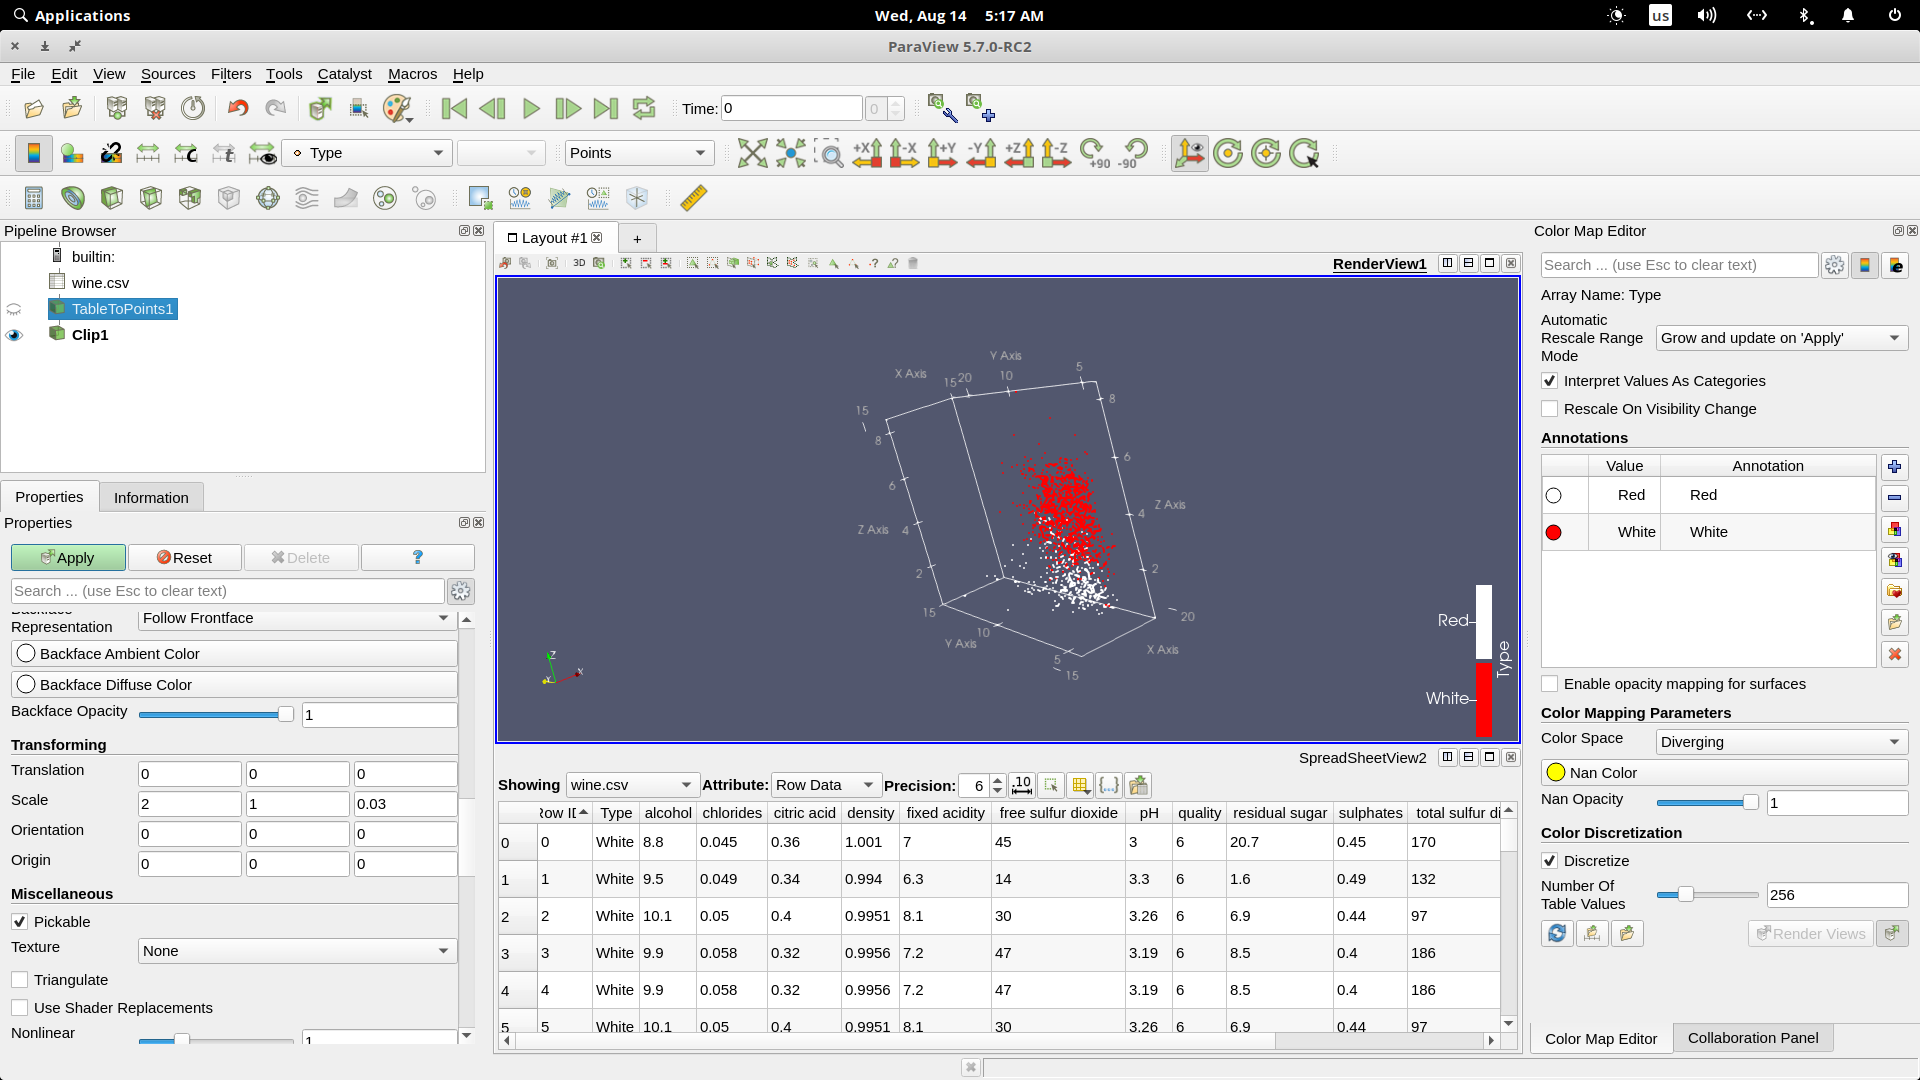
\includegraphics[scale=0.18]{images/paraview}
\caption{Result of our example workflow.}
\label{fig:paraview}
\end{figure}

Other key parts of the user interface include a properties panel, which allows the user to modify parameters of a selected action in the pipeline and the work area where visualizations are drawn. The user is also able to display other panels, which contain further statistical information on loaded dataset. Of particular note is a Color Map panel, which enables the user to choose between various color spaces.\\

There is also a Collaboration panel, which enables multiple users to connect to one another using LAN and share the current state of the work area as well as communicate with one another using text messages. The user roles are clearly defined --- one user acts as a master and has the ability to edit the project, while others act as slaves and cannot interact with the visualization.\\

We will start our usability test by opening our CSV file. ParaView supports a countless amount of input formats. After loading the data, it is analyzed and data types are automatically assigned, the user can choose a delimiter character and specify whether the dataset in question includes headers. To finish the loading process, the user has to click the \emph{Apply} button. After loading the dataset they are presented with a tabular view of it in its entirety.\\

\begin{figure}[!h]
\centering
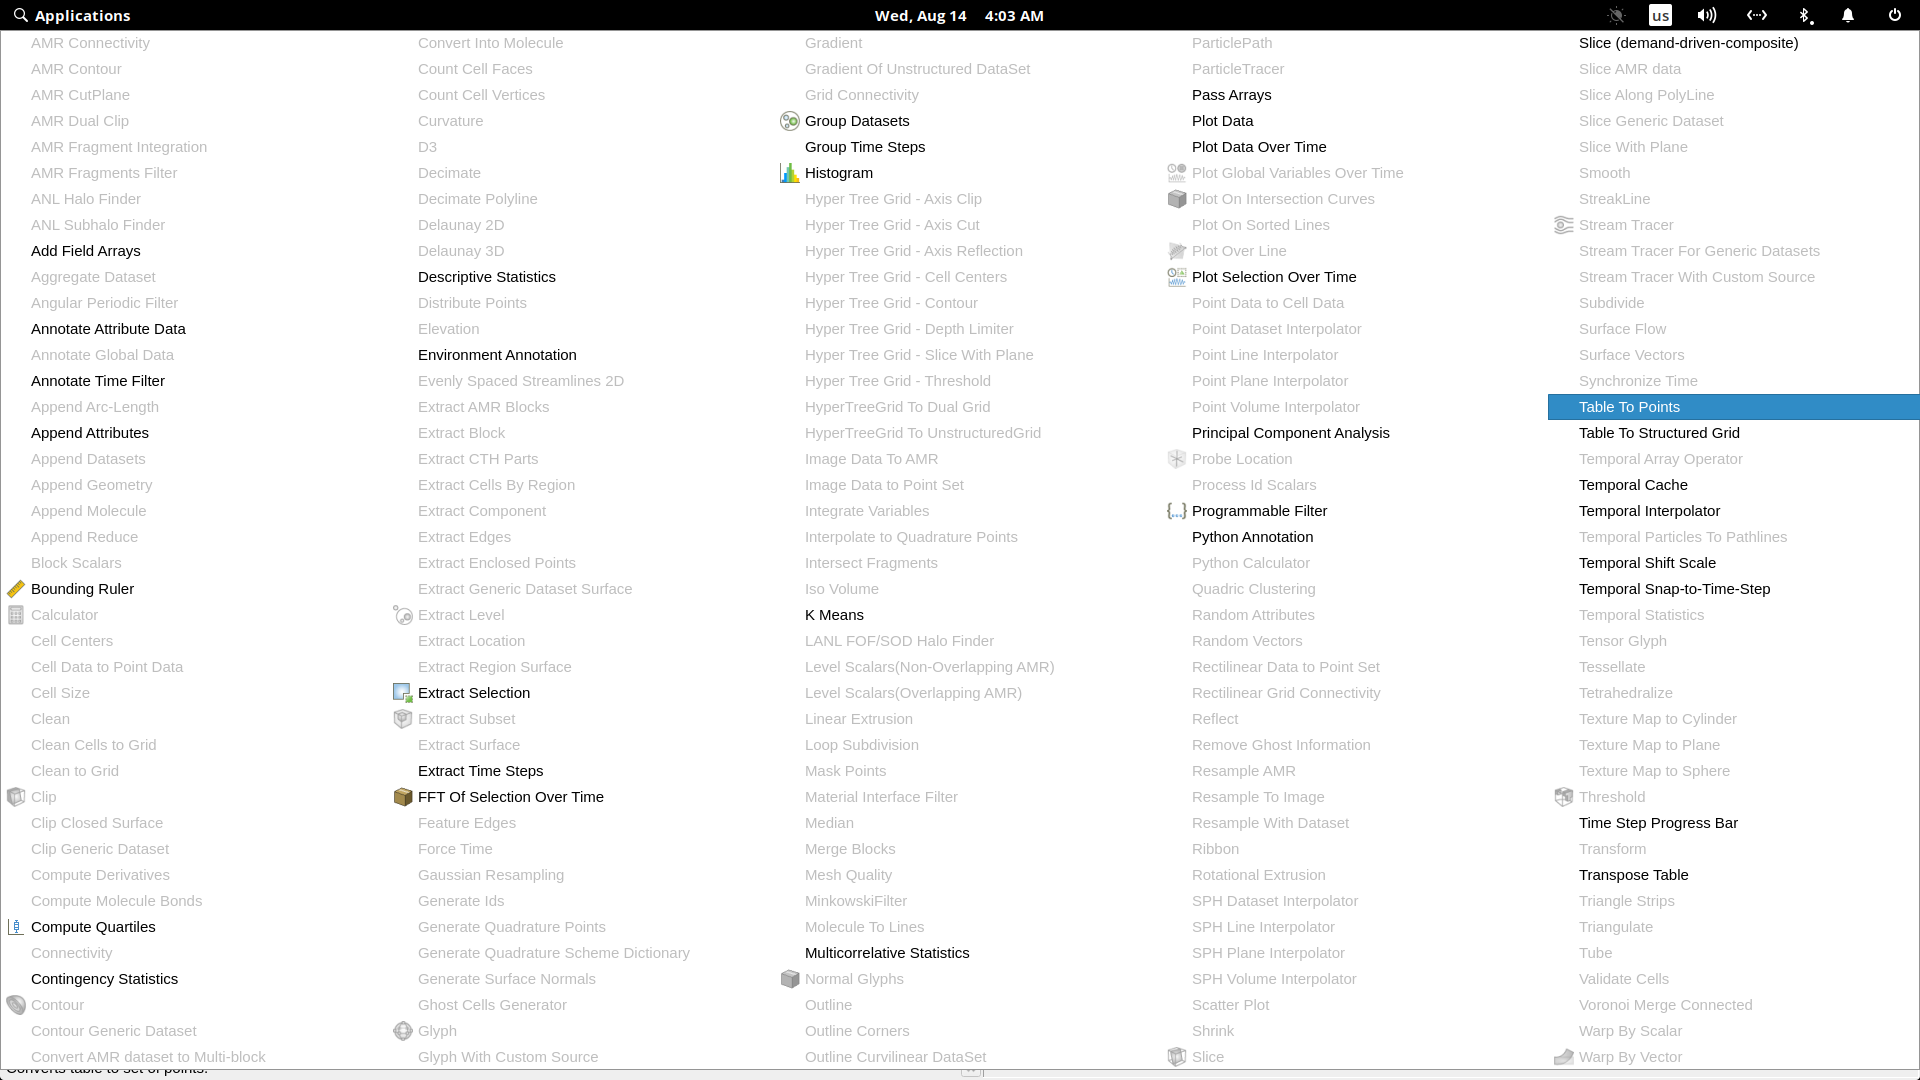
\includegraphics[scale=0.18]{images/paraview_menu}
\caption{Menu listing all available filters.}
\label{fig:paraviewmenu}
\end{figure}

Next, we need to create a scatter plot. This is done in a very convoluted fashion by first selecting the dataset action in the pipeline browser and then opening up a menu via \emph{Filters \textrightarrow{} Alphabetical}. This menu takes up the entirety of the screen and contains many seemingly unrelated actions. An obvious choice for the user would be to select the \emph{Plot Data} option, however they must instead select \emph{Table to Points}.\\

The user is then free to select assignments for spatial axes using a drop down menu and map an attribute onto color in the same fashion. Clicking \emph{Apply} and afterwards clicking the eye icon next to the filter renders the plot.\\

\newpage

The plot appears to be stretched, so we have to scale it by first pressing the cog icon to enable advanced options, and then modifying scale values for each axis in the \emph{Transforming} section by typing in random values until we are satisfied with the look of our plot.\\

As points are very small when we zoom in the plot, we set \emph{Point Size} to a larger number. In order to be able to rotate the plot, we need to reset the pivot by pressing the \emph{Zoom To Data} button in ParaView's toolbar.\\

The next step is to slice the data by using the clip filter. We add the filter using \emph{Filters \textrightarrow{} Alphabetical \textrightarrow{} Clip}. It is appended to the end of our pipeline, however we need to copy the transform values to the new filter. Finally, we select the desired cutting plane using \emph{X/Y/Z Normal} buttons and drag the plane to a position that we would like. In order to view original axes, we select the result of \emph{Table to Points} filter in our pipeline.\\

The following table lists all KLM operations necessary to complete our task. The total time to complete our tasks is 75.74 seconds. Overall, ParaView seems like a powerful tool, albeit with a very convoluted user interface. The tool's tutorial guide contains 159 pages, although it covers advanced functionality in its later chapters.\\

\begin{table}[]
\centering
\caption{Listing of KLM operations for ParaView.}
\label{klm-paraview}
\scalebox{0.7}{
\begin{tabular}{lll}
Operator & Description & Time (s)\\
M & Initiate opening a file & 1.35\\
M & Find file open button & 1.35\\
PB & Point at the button and press it & 1.3\\
PB & Select file and double click it & 1.3\\
M & Find properties panel & 1.35\\
PB & Point on \emph{Apply} button and press it & 1.3\\
M & Initiate plot addition & 1.35\\
PBPPB & Open up \emph{Filters} menu, navigate to \emph{Alphabetical \textrightarrow{} Table to Points} & 3.7\\
M & Find \emph{Properties} section of \emph{Properties} panel & 1.35\\
3*(PBPB) & Select assignments from dropdown & 7.8\\
M & Find \emph{Coloring} section of \emph{Properties} panel & 1.35\\
PBPB & Select an assignment from dropdown & 2.6\\
M & Find \emph{Styling} section of \emph{Properties} panel & 1.35\\
PBHKH & Change value of point size & 2.38\\
PB & Click on the eye icon to display filter & 1.3\\
M & Find \emph{Transforming} section of \emph{Properties} panel & 1.35\\
6*(PBHKKKH) & Guess transform scales that make length of plot's axes equal & 17.64\\
MPB & Find \emph{Zoom to Data} button and press it & 1.3\\
PBPPB & \emph{Filters \textrightarrow{} Alphabetical \textrightarrow{} Clip} & 3.7\\
PBPB & Click on the eye icon next to two recently added filters & 2.6\\
M & Find \emph{Transforming} section of \emph{Properties} panel & 1.35\\
3x(PBHKKKH) & Fill in scale values from the previous filter & 8.82\\
M & Find \emph{Plane parameters} section of \emph{Properties} panel & 1.35\\
PB & Point and click on desired normal button to create a cutting plane & 1.3\\
PBPB & Drag the cutting plane to desired position & 2.6\\
PB & Click on \emph{Apply} & 1.3\\
PB & Select original filter to display its axes & 1.3
\end{tabular}
}
\end{table}

\subsubsection{Tableau}

Tableau is a commonly used software for business intelligence. It allows the user to load data by opening a local file (CSV, JSON, Excel spreadsheet) or connecting to a database (MSSQL, Oracle, MySQL, Amazon Redshift and more). The number of database integrations is much larger than the number of supported types of local files indicative of the product's focus on enterprises and big data. The desktop application is available for Windows and macOS.\cite{tableau}\\

\begin{figure}[!h]
\centering
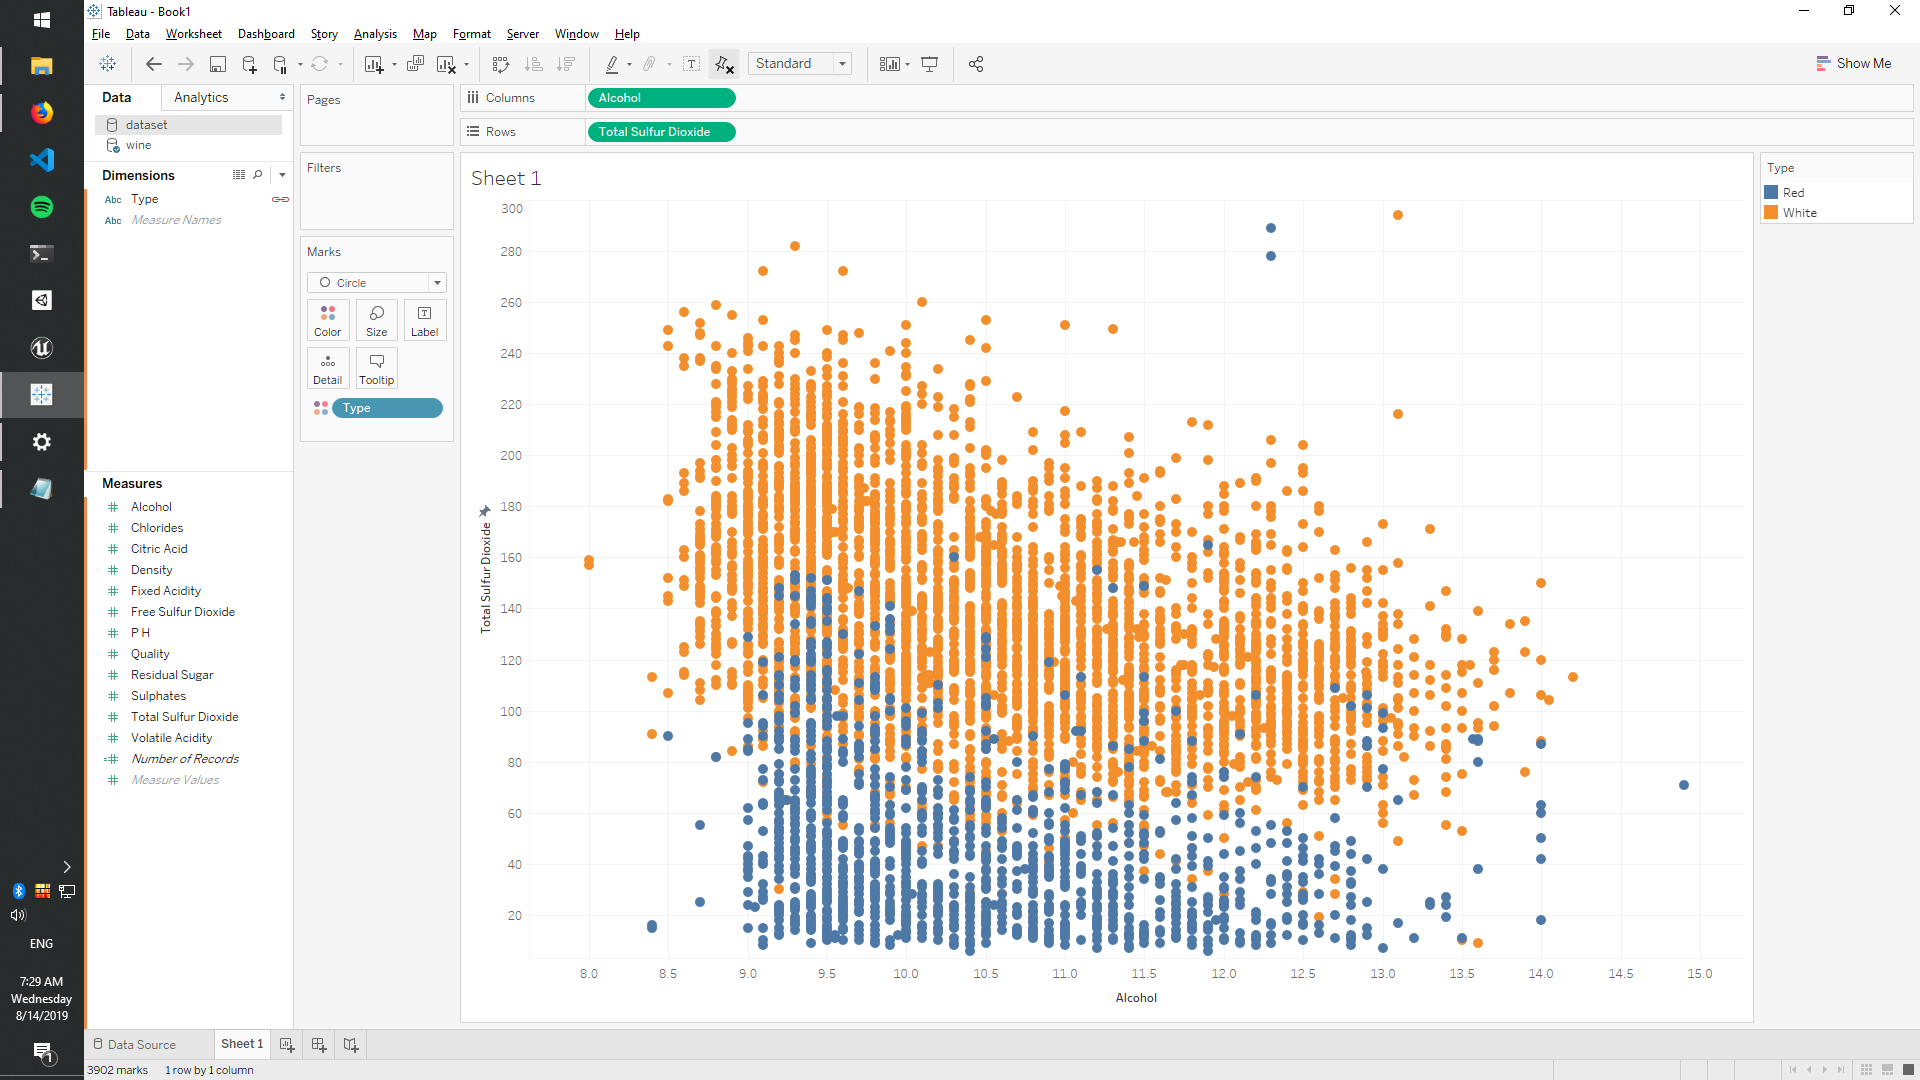
\includegraphics[scale=0.25]{images/tableau_sheet}
\caption{Tableau's sheet view.}
\label{fig:tableausheet}
\end{figure}

The company also offers a product called Tableau Server which enables the users to store their data online using either a publicly hosted service or an on--premises server.\\

The client software includes a very straightforward and easy--to--use interface. The user loads a dataset and is presented with a tabular view. Data types are automatically detected, as is the column delimiter (in the case of CSV files). In this view, the user is also able to pre--filter data by selecting a threshold and filling in null values. They are then able to create a \emph{sheet}, a metaphor commonly used in spreadsheet software. The user then selects attributes they would like to use by dragging them into a \emph{Dimensions} list and afterwards can map them onto rows, columns and non--spatial features of the two--dimensional scatter plot.\\

\newpage

Unfortunately, as of version 2019.2.2, Tableau does not have native support for three-dimensional plots. There is a workaround for creating pseudo--3D plots, but it requires the use of a SQL database and is not user--friendly at all, being more of a hack than a proper solution.\cite{tableau3d}\\

\begin{figure}[!h]
\centering
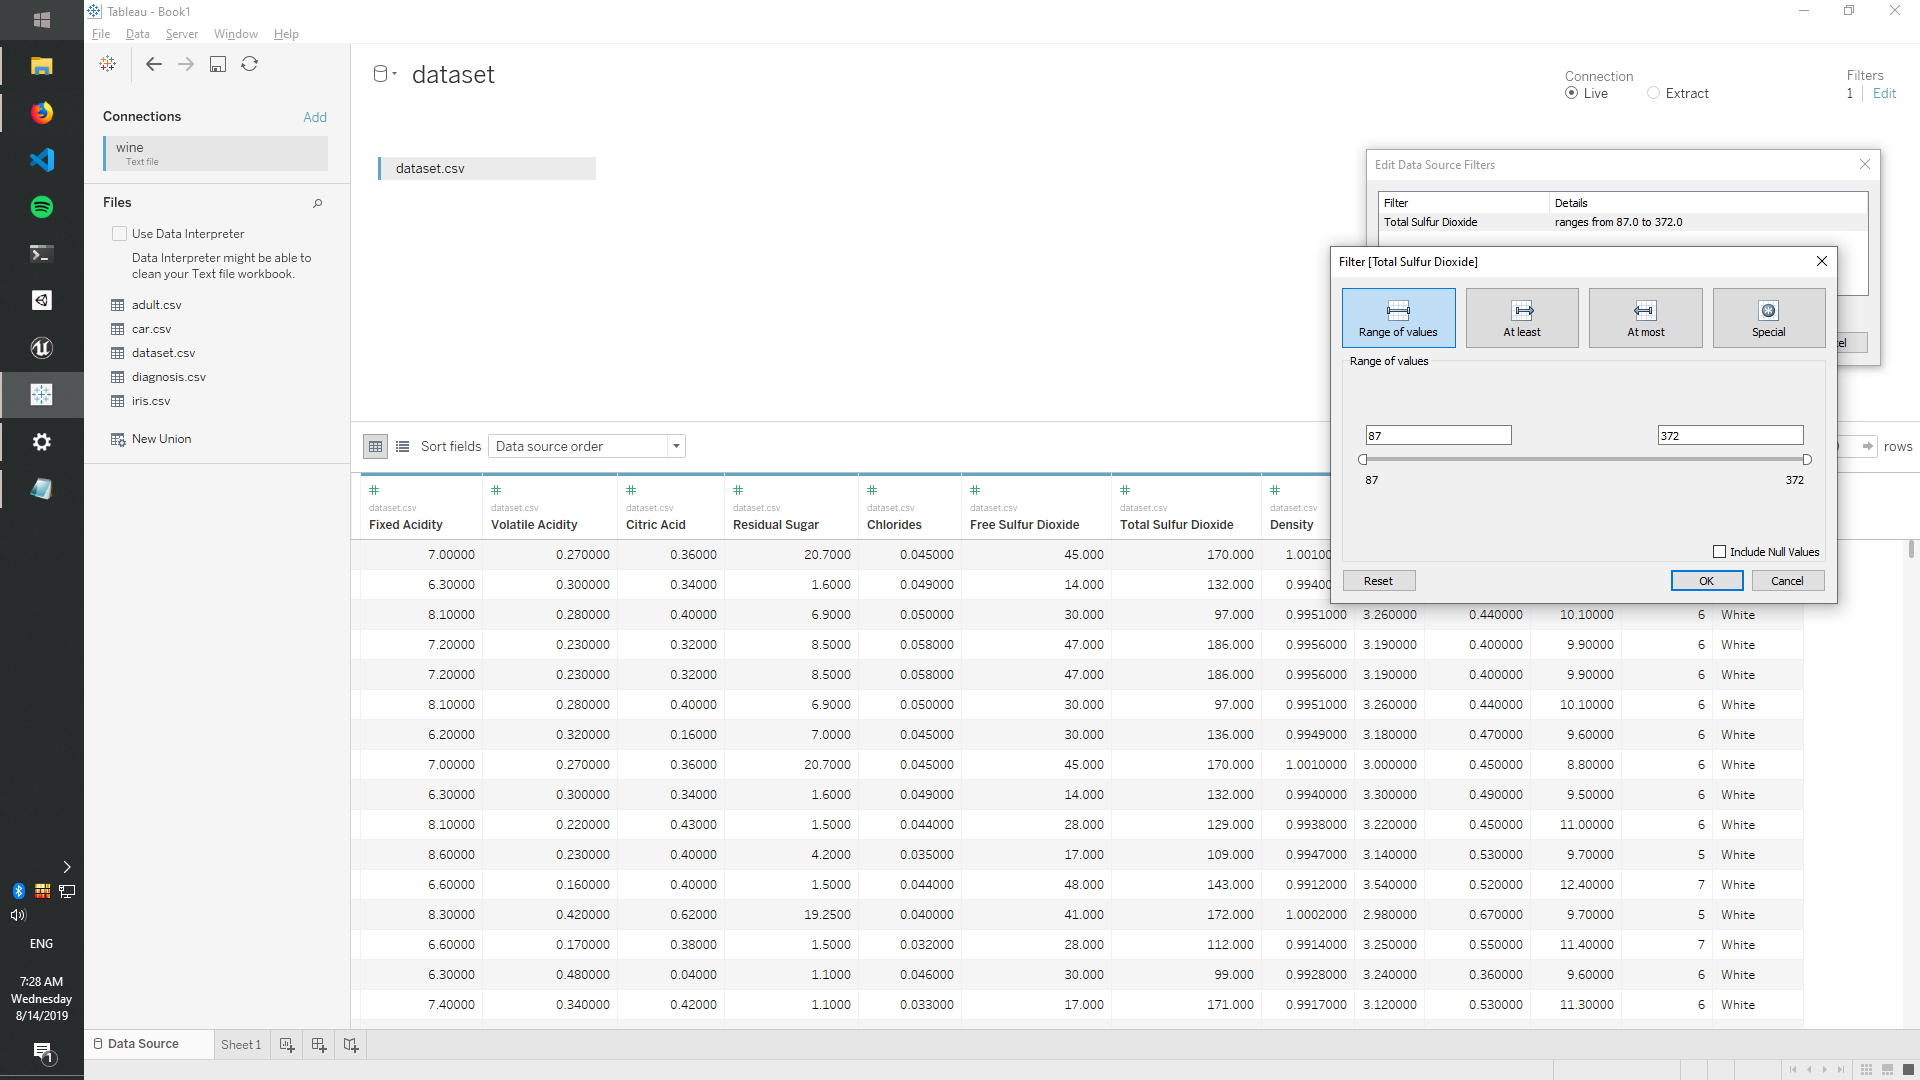
\includegraphics[scale=0.25]{images/tableau_edit}
\caption{Tableau's edit view.}
\label{fig:tableauedit}
\end{figure}

The following table lists all KLM operations necessary to complete a simplified task of creating a two--dimensional scatter plot.\\

\begin{table}[!h]
\centering
\caption{Listing of KLM operations for Tableau.}
\label{klm-tableau}
\scalebox{0.7}{
\begin{tabular}{lll}
Operator & Description & Time (s)\\
M & Initiate opening a file & 1.35\\
M & Find \emph{More...} button on sidebar & 1.35\\
PB & Point at the button and press it & 1.3\\
PB & Select file and double click it & 1.3\\
M & Locate \emph{Sheet1} tab & 1.35\\
PB & Point at the tab and press it & 1.3\\
M & Locate \emph{Measures} and \emph{Dimensions} lists & 1.35\\
3*(PBPB) & Move attributes we want to display from \emph{Measures} to \emph{Dimensions} & 7.8\\
M & Locate plot dimension settings & 1.35\\
2*(PBPB) & Move spatial attributes from \emph{Dimensions} list to \emph{Columns} and \emph{Plots} respectively & 5.2\\
2*(PBPB) & Click on both assignments and select \emph{Continuous} from dropdown menu & 5.2\\
PBPB & Move one attribute from \emph{Dimensions} onto \emph{Color} subsection of \emph{Marks} panel & 2.6\\
M & Locate axis we want to slice & 1.35\\
PBPB & Right click on the axis and select \emph{Edit Axis} from dropdown & 2.6\\
PB & Select \emph{Fixed} radio button & 1.3\\
PBHKKKH & Input desired value to \emph{Fixed end} textbox & 2.94\\
PB & Close the modal & 1.3
\end{tabular}
}
\end{table}

The total time to complete our tasks is 40.94 seconds, half the time of a similar workflow in ParaView. However, we have only been able to create a two--dimensional scatter plot due to software's limitations.

\subsection{Benefits of virtual reality}

We believe that virtual reality has the potential to enhance the visualization experience. Let us explore several reasons why.

\subsubsection{Stereoscopic view, 6DOF}

Head--mounted displays (HMD) are by design stereoscopic. One study compared error rates on a conventional monitor against a stereoscopic solution with eye separation (interpupilary distance, IPD) of 6.4 cm. It also focused on the benefits of dynamic motion for perception.\\

The findings were that the use of both dynamic motion and stereoscopy significantly reduced error rates (by 10\% in inexperienced participants, n=14 and 15--30\% in experienced participants, n=2). Combination of these two methods led to further improvement.\cite{ware}\\

With modern HMDs we can leverage both of these methods as 6 degrees of freedom (6DOF) headsets allow the user to freely position their head in space, simulating motion.

\subsubsection{Spatial interface}

Researchers and designers alike have been looking at replacing the traditional Windows--Icons--Menus--Pointing (WIMP) desktop metaphors with 3D alternatives since the early 90s. The new interfaces instead rely on hand gestures and speech recognition to navigate around 3D space. One article from the era argues that users are frustrated by many layers of \emph{point and click} and visual clutter that is common with WIMP UIs and discusses the limitations of relying exclusively on the sense of sight. The author prophesizes rise of virtual reality and proceeds to discuss potential applications.\cite{wimp}\\

Innovative examples such as Google Earth VR prove that well--designed spatial interfaces have the potential to make UI more intuitive, especially to first--time users.\cite{earthux}

\subsubsection{Immersive analytics}

The full use of one's visual field as well as senses of touch (through force feedback) and spatial sound allows the user to fully immerse themselves into their data, which has potential to improve their concentration. Furthermore, they have the ability to invite other users into their virtual space, which allows for multi--user interactions with plots inside the space.

\section{Existing products}

In this part we will focus on analyzing existing VR--enabled visualization tools. Emphasis is given on select features that author perceives as relevant. We will explore data support to see how we can load data onto the platform, as well as options for extensibility via plugins. Due to the rise of mobile HMDs, we will look at how well they are supported in each product. From the feature set, we will focus on machine learning capabilities and collaboration features. Lastly, we will take a quick look at business models of companies that develop these applications and check availability of editions aimed at end consumers and/or academia.

\subsection{Virtualitics}

Virtualitics aims to combine the benefits of high--dimensional visualization in VR with those of AI--driven analysis.\cite{virtualitics} Virtualitics includes a Windows application for loading, editing and visualizing data in both desktop mode and VR, the later enables the user to visualize data in an immersive environment as well as to collaborate with other users who are represented as avatars. Virtualitics also offers a Python API, which enables programmers to implement an integration into their applications. This API is available in the Python repository under a FOSS license (MIT).\cite{pyvip}\\

\begin{figure}[!h]
\centering
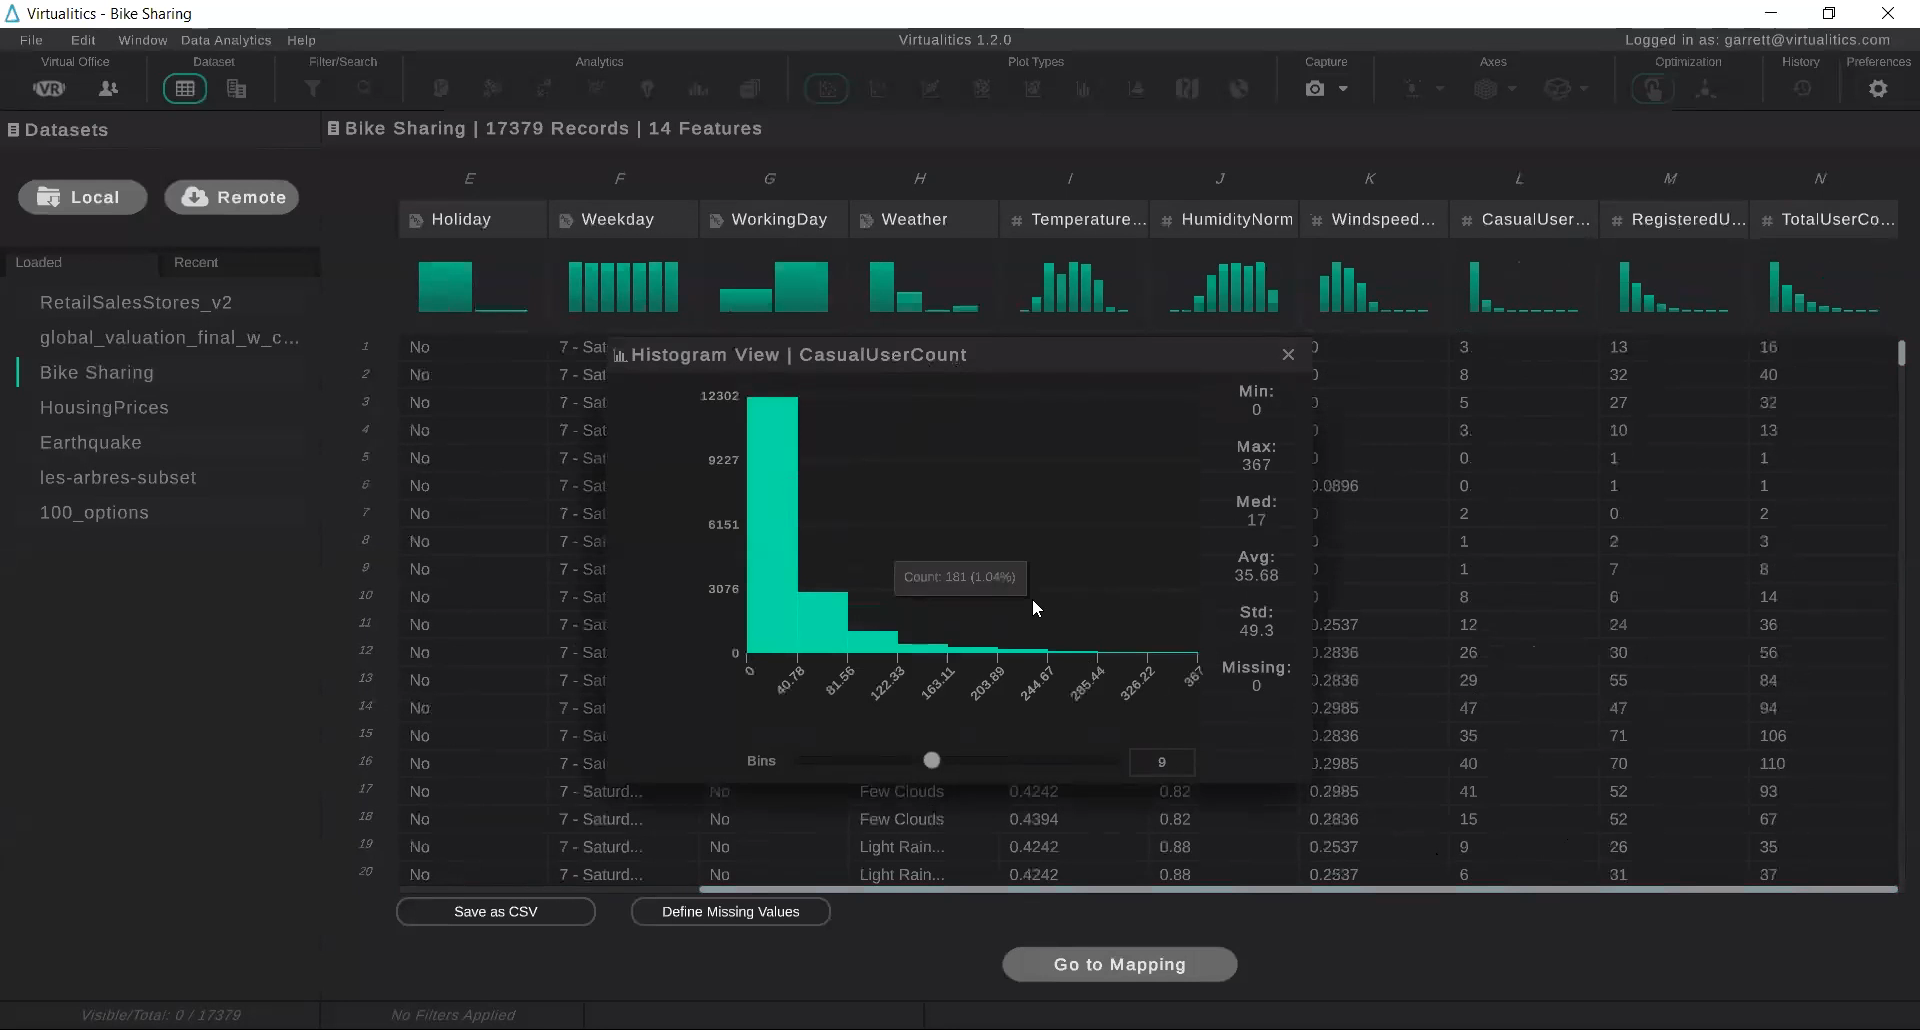
\includegraphics[scale=0.18]{images/virtualitics_spreadsheet}
\caption{Spreadsheet view in Virtualitics's desktop application.\cite{virtualiticsvideo}}
\label{fig:virtualiticssheet}
\end{figure}

The interface of Virtualitics's desktop application bears resemblance to Tableau. Data can be loaded from either a local file or a remote database. It includes a \emph{spreadsheet view}, which shows loaded data in a tabular form with histograms and basic statistical information such as mean and median. The user is able to filter data and fill in missing values.\\

Afterwards, they are able to switch into the \emph{mapping view}, which allows them to map attributes onto dimensions. A unique feature called \emph{smart mapping} offers the user a selection of attributes that are calculated to be the most important in the dataset. The user can also toggle between multiple plot types.\\

\begin{figure}[!h]
\centering
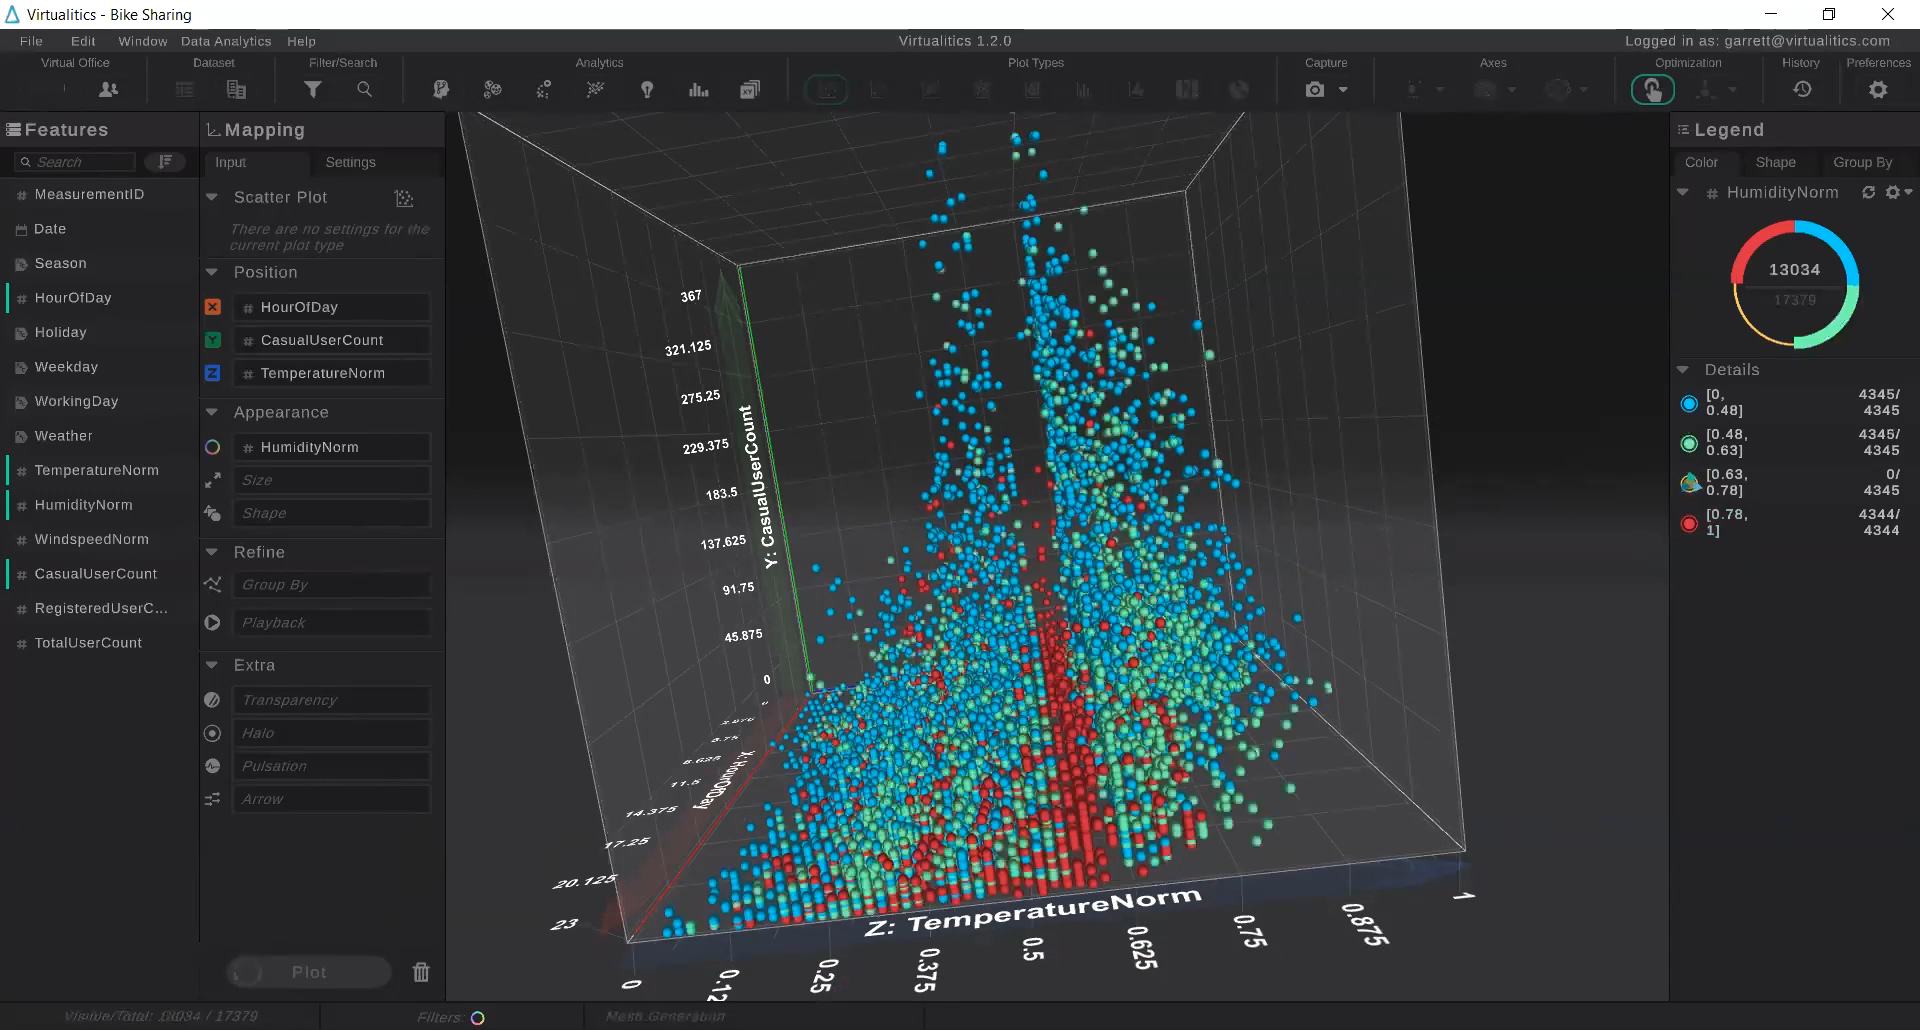
\includegraphics[scale=0.18]{images/virtualitics_mapping}
\caption{Mapping view in Virtualitics's desktop application.\cite{virtualiticsvideo}}
\label{fig:virtualiticsmap}
\end{figure}

The VR component dubbed \emph{Virtual Office} allows the user to interact with plots they have defined in the \emph{mapping view} in VR. They are able to access key features of the desktop application using flat panels which look the same as they do in desktop mode. The user can interact with one 3D plot at a time, which is located at the center of the virtual space with 2D plots surrounding the user and offering more insight. The software includes a collaboration feature, enabling the user to invite other stakeholders into their virtual environment.\\

Virtualitics's Python API enables the user to connect to a running instance of the desktop application and load data from a Pandas data table as well as access certain analytics and visualization features straight from their code.\\

\begin{figure}[!h]
\centering
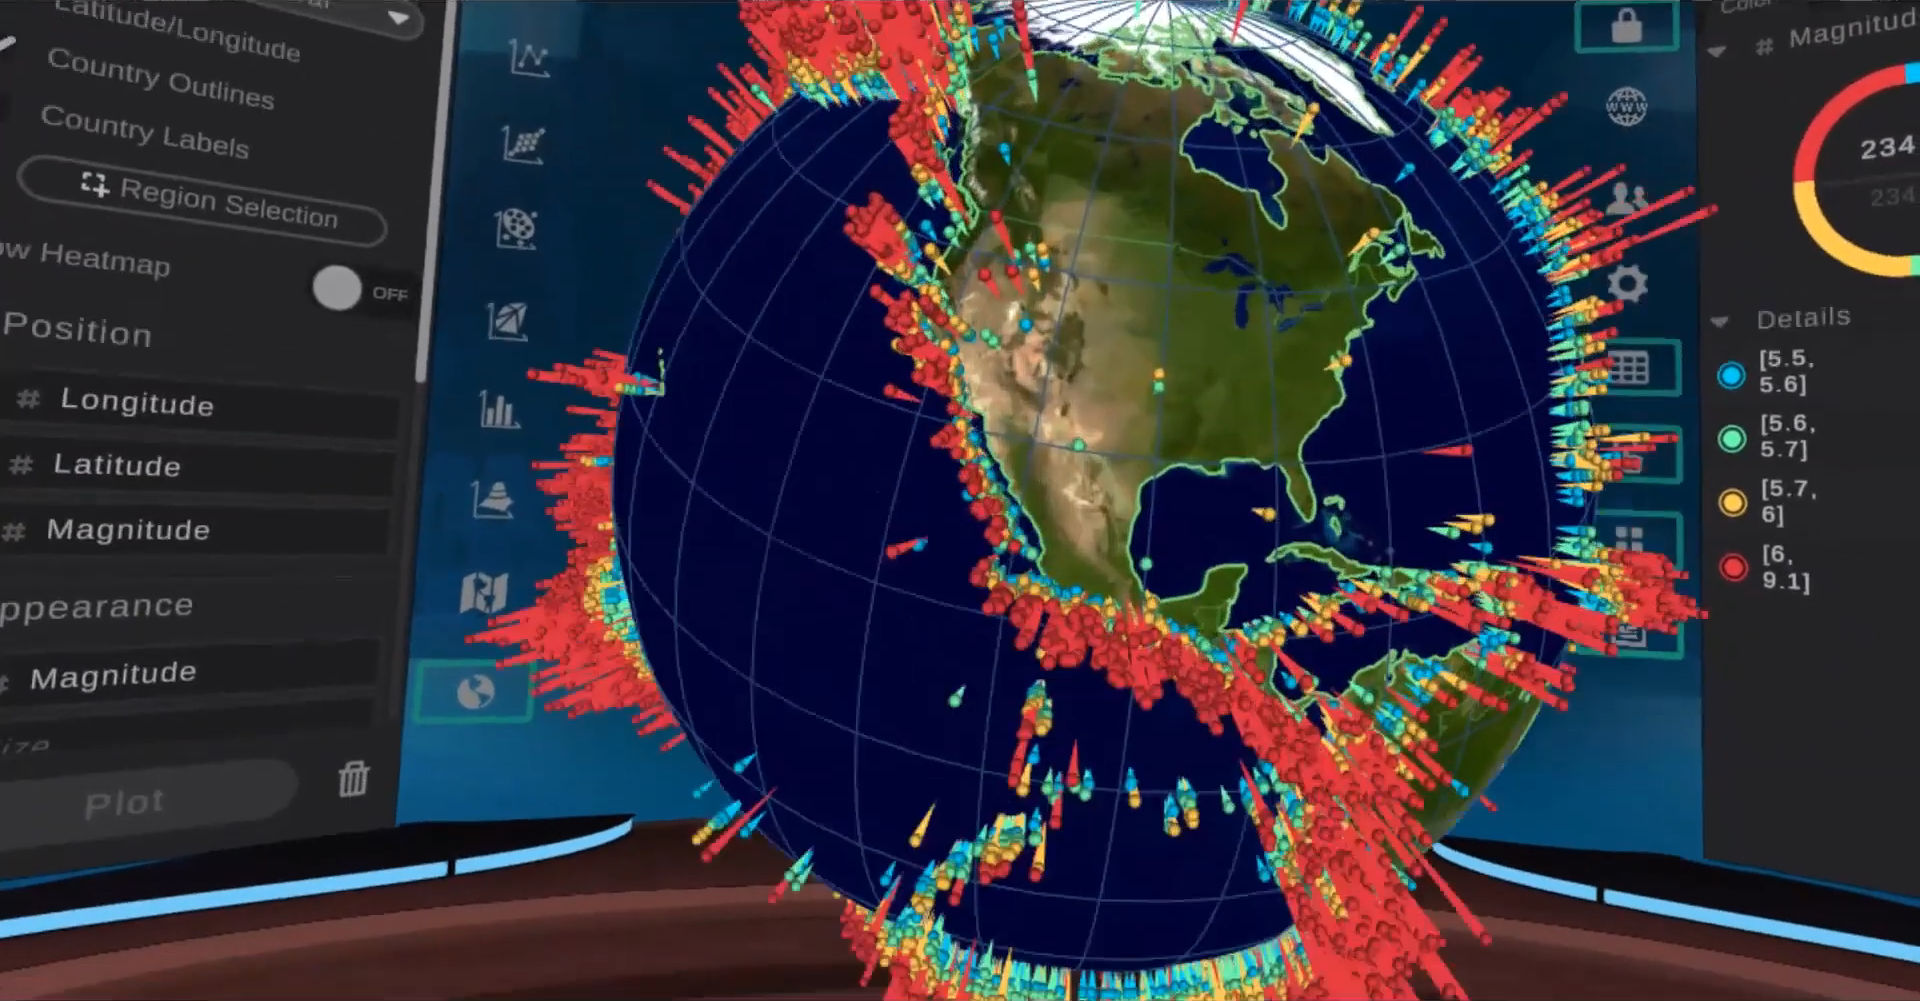
\includegraphics[scale=0.18]{images/virtualitics_vr}
\caption{Virtualitics's VR interface.\cite{virtualiticsvideo}}
\label{fig:virtualiticsvr}
\end{figure}

Out of the three products that we have analyzed, Virtualitics seems to be the most advanced. It offers a very clean task--driven user interface, powerful tools for analytics, mobile support for Oculus Quest, large number of integrations with an open--source Python API and collaboration features. Negatives include proprietary nature of all other components, which require users to resort to the aforementioned Python API, lack of support for 3DOF headsets such as Oculus Go or Google Daydream, VR interface that is perhaps too similar to its desktop counterpart and does not fully utilize the capabilities of room scale VR and, as with all other products mentioned, lack of any consumer or academic version.

\subsection{LookVR}

LookVR is a virtual reality tool for exploring data that is part of Looker, an enterprise business analytics platform.\cite{lookvr} Looker enables its customers to connect to more than 50 types of databases. Their BI platform can be accessed via a web browser, a demo of an example dashboard is available.\cite{lookerdash} LookVR enables the user to access 3D scatter plots, bar plots as well as more unorthodox plot types hosted on Looker. There does not seem to be any interactivity at all outside of selecting a plot. The software allows the user to push a cartoon--like \emph{big data} button in order to enlarge the visualized plot.\\

\begin{figure}[!h]
\centering
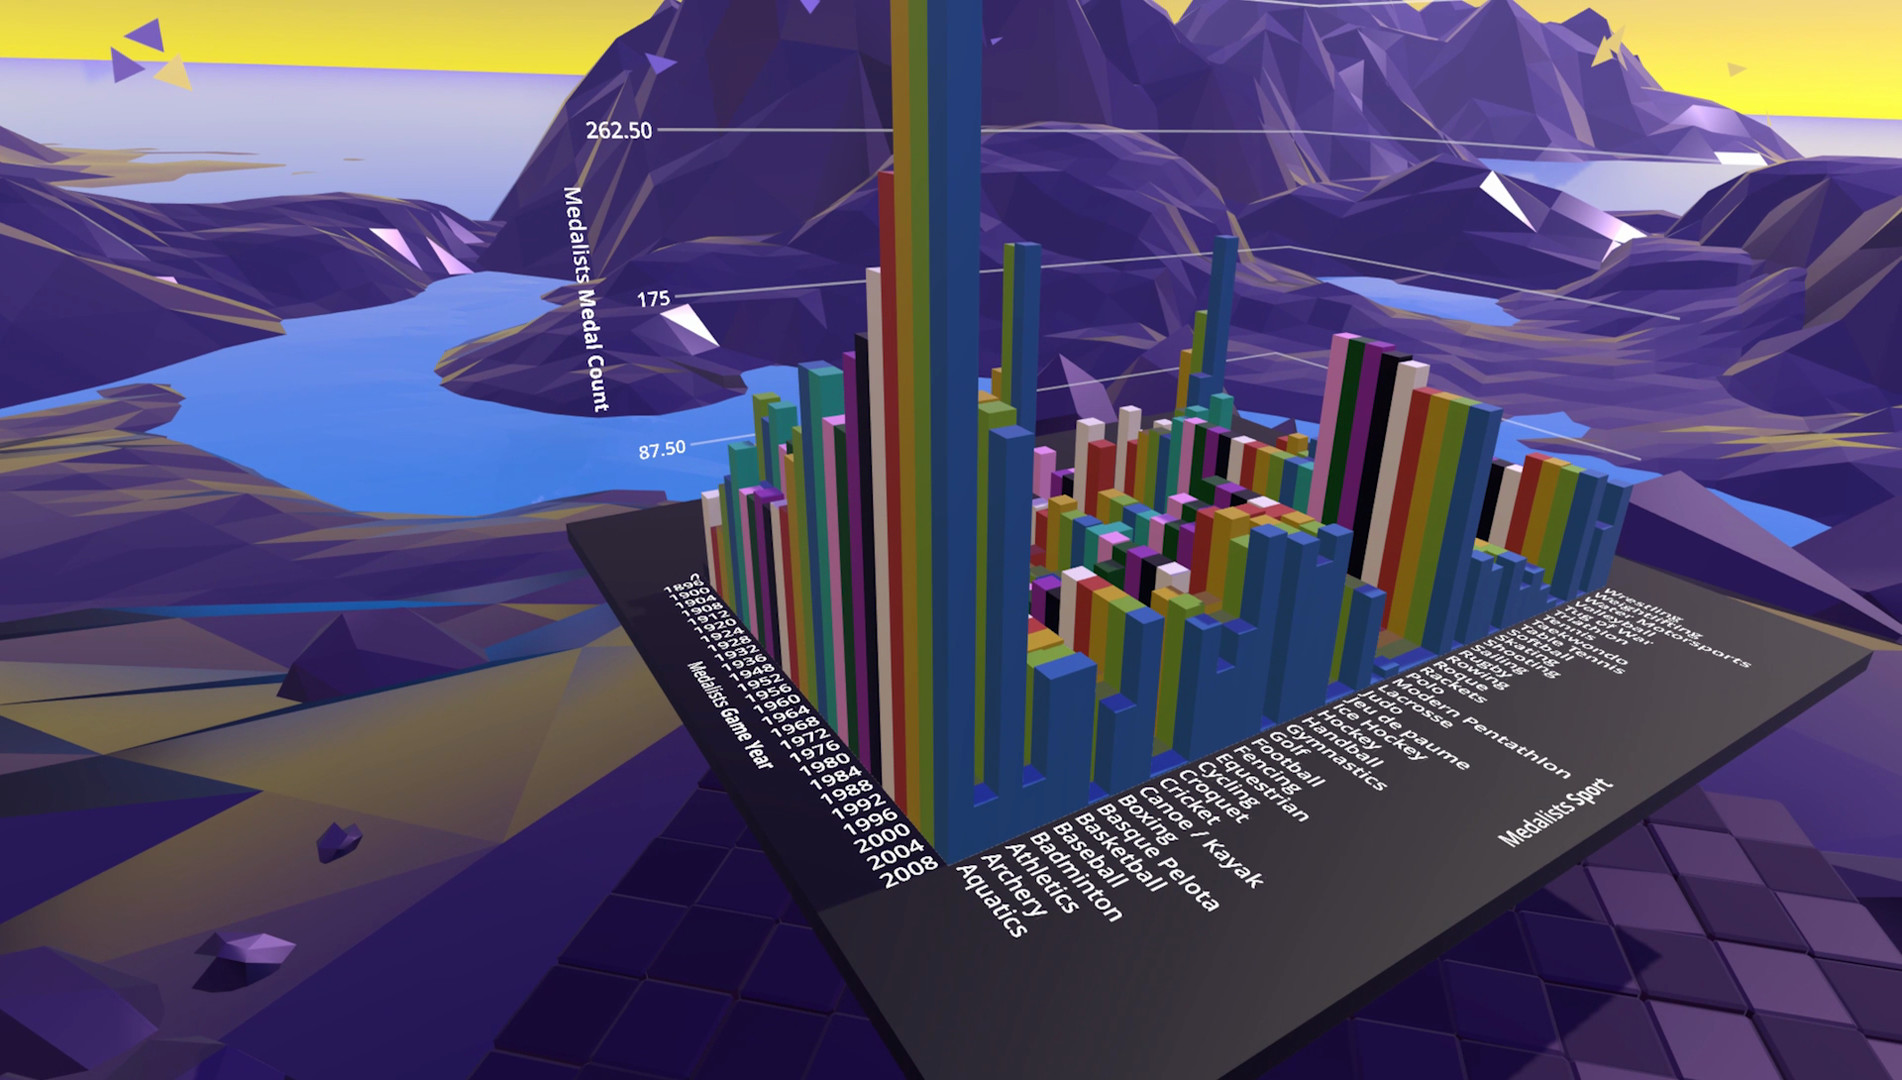
\includegraphics[scale=0.18]{images/lookvr}
\caption{LookVR's user interface.\cite{lookvrsteam}}
\label{fig:lookvr}
\end{figure}

LookVR is available for free via Steam.\cite{lookvrsteam} If the user's company has access to Looker, they may log in using their credentials, otherwise a small selection of plots is available as a sample. Unfortunately, all of our attempts to load sample data have ended unsuccessfully.\\

When it comes to LookVR's feature set, it is rather basic. The amount of available plot types is small, there is no support for mobile HMDs, no extensibility or FOSS components and although it is distributed for free via Steam, the requirement of a Looker license does not allow non--enterprise customers to utilize the product.\\

\subsection{3Data}

Austin--based startup 3Data started as a 2016 prototype called DataVizVR.\cite{datavizvroculus} As of August 2019, this demo is still available via Oculus Store. The demo features a number of preloaded datasets and enables the user to interact with a single plot via a very spartan user interface. Since then, the product has matured, offering various plot types including terrain maps.\cite{3data}\\

\begin{figure}[!h]
\centering
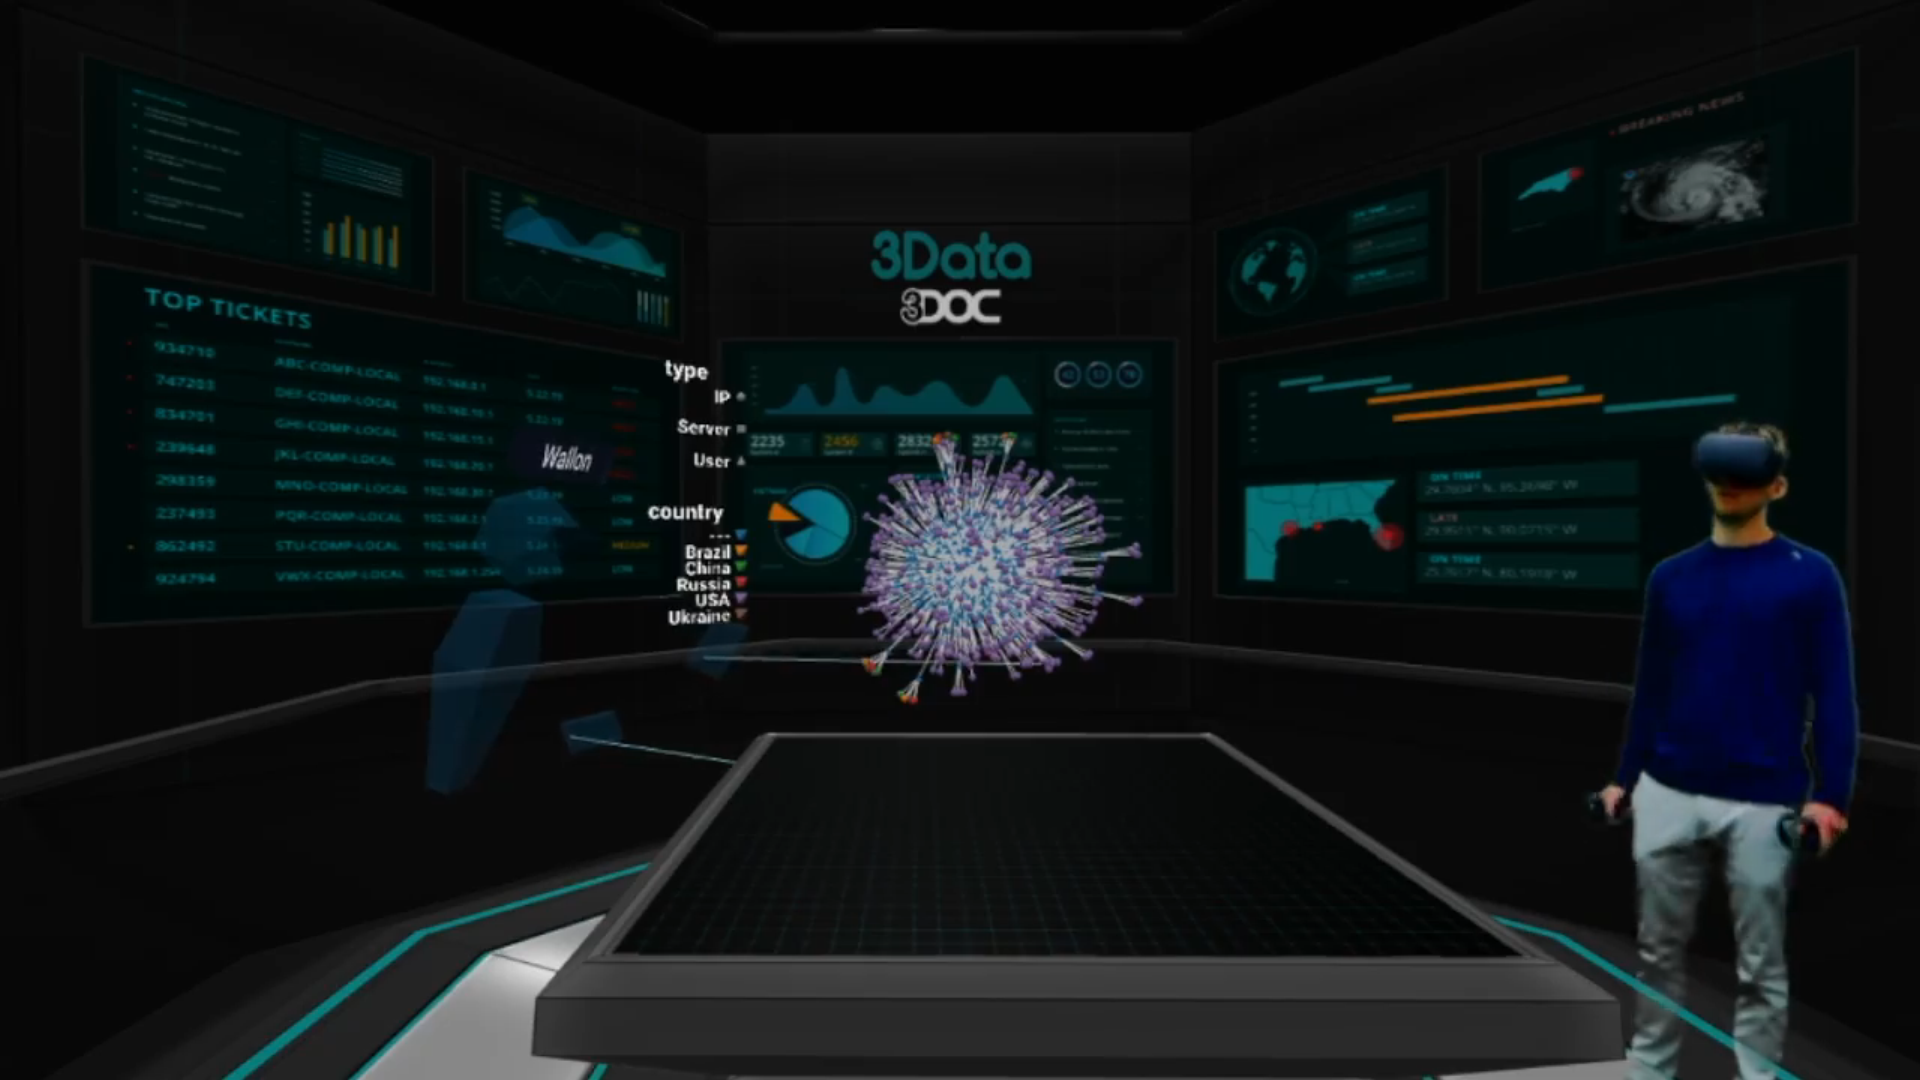
\includegraphics[scale=0.18]{images/3data}
\caption{3Data's immersive VR environment.\cite{3datavideo}}
\label{fig:3data}
\end{figure}

Its user interface, dubbed \emph{3Data Operations Center}, seems similar to Virtualitics with a plot front and center and details surrounding the user in a virtual room, albeit slightly less polished. Like its competitor, 3Data also offers collaboration features.\\

The product is sold solely to companies as an applications suite called \emph{3Data Power Office}, which in addition to the VR viewer includes tools for creating immersive presentations and collaboration with other stakeholders. Datasets can be self--hosted, 3Data promises direct connection to databases and existing BI tools.\cite{3datasuite}\\

A defining feature of 3Data is its ability to run across multiple classes of devices. The visualization component makes use of WebVR specification, which enables it to run on VR/AR headsets, handheld mobile devices and personal computers in both 2D and immersive modes.\cite{webvr} 3Data does not seem to offer a dataset editing tool of its own, relying instead on third--party applications.\\

\newpage

At the moment, the product does not support any analytical features, however support for \emph{IBM Watson} is coming soon. After a detailed inspection, we concluded that there are no FOSS components whatsoever.

\subsection{Summary}

Unfortunately, due to the enterprise nature of analyzed products and lack of a consumer/academic license or trial version, we have not been able to test these applications ourselves. The following chart compares key features of analyzed products.\\

\begin{figure}[!h]
\centering
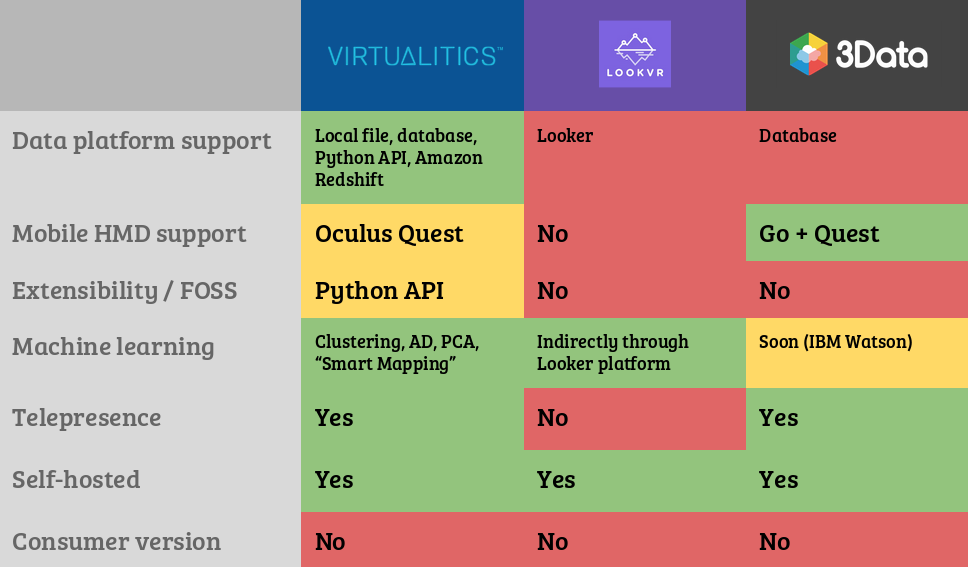
\includegraphics[scale=0.35]{images/comparison}
\caption{Comparison of VR data visualization applications.}
\label{fig:comparison}
\end{figure}

\section{Design}

In this chapter we discuss the structure of our application suite, introduce some key features and go over certain technical and design challenges we had to overcome.

\subsection{Goal}

The goal of our research is to create a virtual reality visualization environment that is accessible to everyone, is easily extensible by outside developers and works on 3DOF and 6DOF HMDs, no matter whether they are connected to a personal computer or standalone. Different control styles should be taken into account when designing interactions.

\subsection{Feature selection}

We have selected a number of features to implement for our first prototype, which was made in the space of 4 months (one academic semester). These include the ability to load comma--delimited CSV files into the environment, ability to update existing datasets by either overwriting the existing copy or appending a new copy (\emph{versioning}), letting the user perform basic editing operations such as renaming dataset attributes, setting their data type and missing value setting and a basic dataset sharing feature.\\

The user should also be able to create scatter plots, position them freely around the virtual environment, adjust their rotation and scale, specify bounds for each spatial axis (\emph{slicing}), assign dataset attributes onto spatial axes and non--spatial features such as color and size and view basic dataset metadata and statistics of attributes contained within said dataset.\\

Lastly, there should be integration support for popular programming languages that allows programmers to create or update datasets from their programming environment of choice. Since we cannot cater to all, we should provide the ability for outside developers to build their own integrations for other programming languages or environments.

\subsection{Component design}

We have decided to divide our environment into three distinct components -- plugins, Manager and Navigator. \emph{Plugins} are API integrations written for different programming languages that allow the user to create a new dataset or update an existing one. \emph{Manager} enables the user to view and edit all of their datasets and also facilitates uploading files from a local computer. \emph{Navigator} allows the user to interact with their data in virtual reality. The following visualization pipeline shows the distribution of tasks among our components.\\

\begin{figure}[!h]
\centering
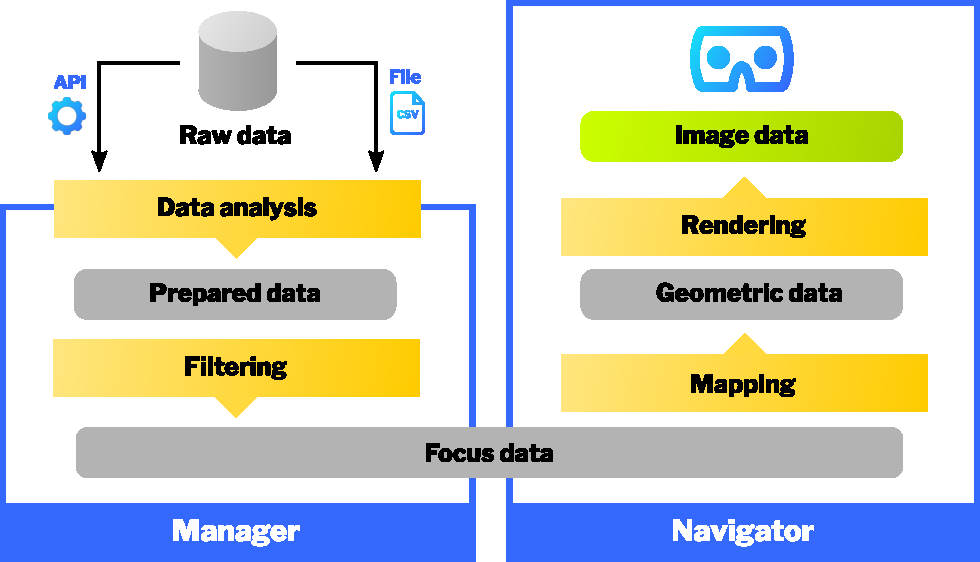
\includegraphics[scale=0.5]{images/pipeline.pdf}
\caption{Adapted version of Haber–McNabb dataflow model for scientific visualization in the context of our environment.\cite{santos}}
\label{fig:dataflow}
\end{figure}

\subsubsection{Plugins}

Plugins are intended for developers or power users to incorporate dataset creation and updating functionality into their applications and scripts. We have implemented integrations for Python and R, as they are the most common programming languages used by data scientists. Manager provides a set of APIs that enable outside developers to create their own integrations and as both Manager and official plugins are open--source\cite{github}, it is a very straightforward process.\\

\newpage

From the user's perspective, the workflow to add or update a dataset is as follows:

\begin{enumerate}
    \item Log into Manager.
    \item Access the create/update dataset modal.
    \item Select programming language or environment.
    \item Copy API key that is unique for user (when creating a dataset) or dataset (when updating an existing dataset).
    \item Import a library in the programming environment of choice.
    \item Insert an applicable command.
    \item Run your program.
\end{enumerate}

The following code snippet showcases the use of plugins for adding a new dataset and updating an existing one in R.

\begin{verbatim}
cyberplot.new(swiss, id = "304a87cff875bc23522557e5beda11ff",
              name = "Swiss Dataset")
cyberplot.update(iris3, id = "09fee44cff6a79cdf2a6176b2ffb1008")
\end{verbatim}

\begin{figure}[!h]
\centering
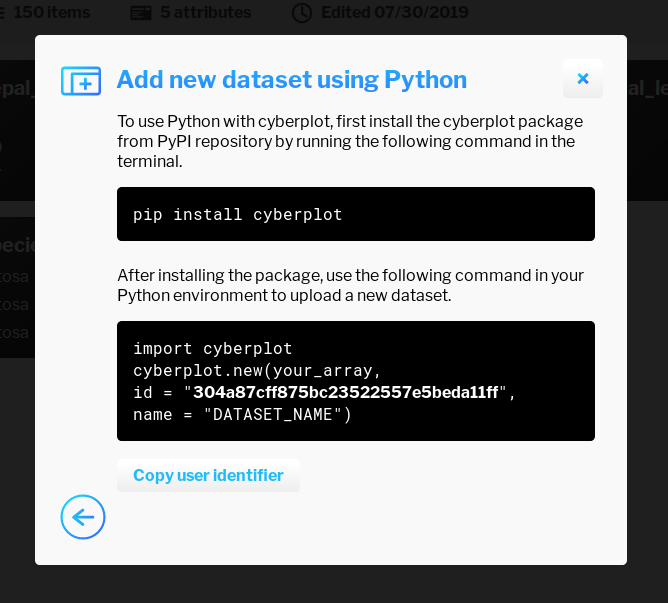
\includegraphics[scale=0.35]{images/manager_python}
\caption{Guide for adding a dataset using Python.}
\label{fig:managerpython}
\end{figure}

\newpage

\subsubsection{Manager}

Manager is the name for our web component. It is meant to be installed on a virtual private server (VPS) and provides dataset storage as well as an interface for users to edit their datasets. In terms of architecture, it forms the central part of our environment, as both plugins and Navigator interacts with its APIs.\\

\begin{figure}[!h]
\centering
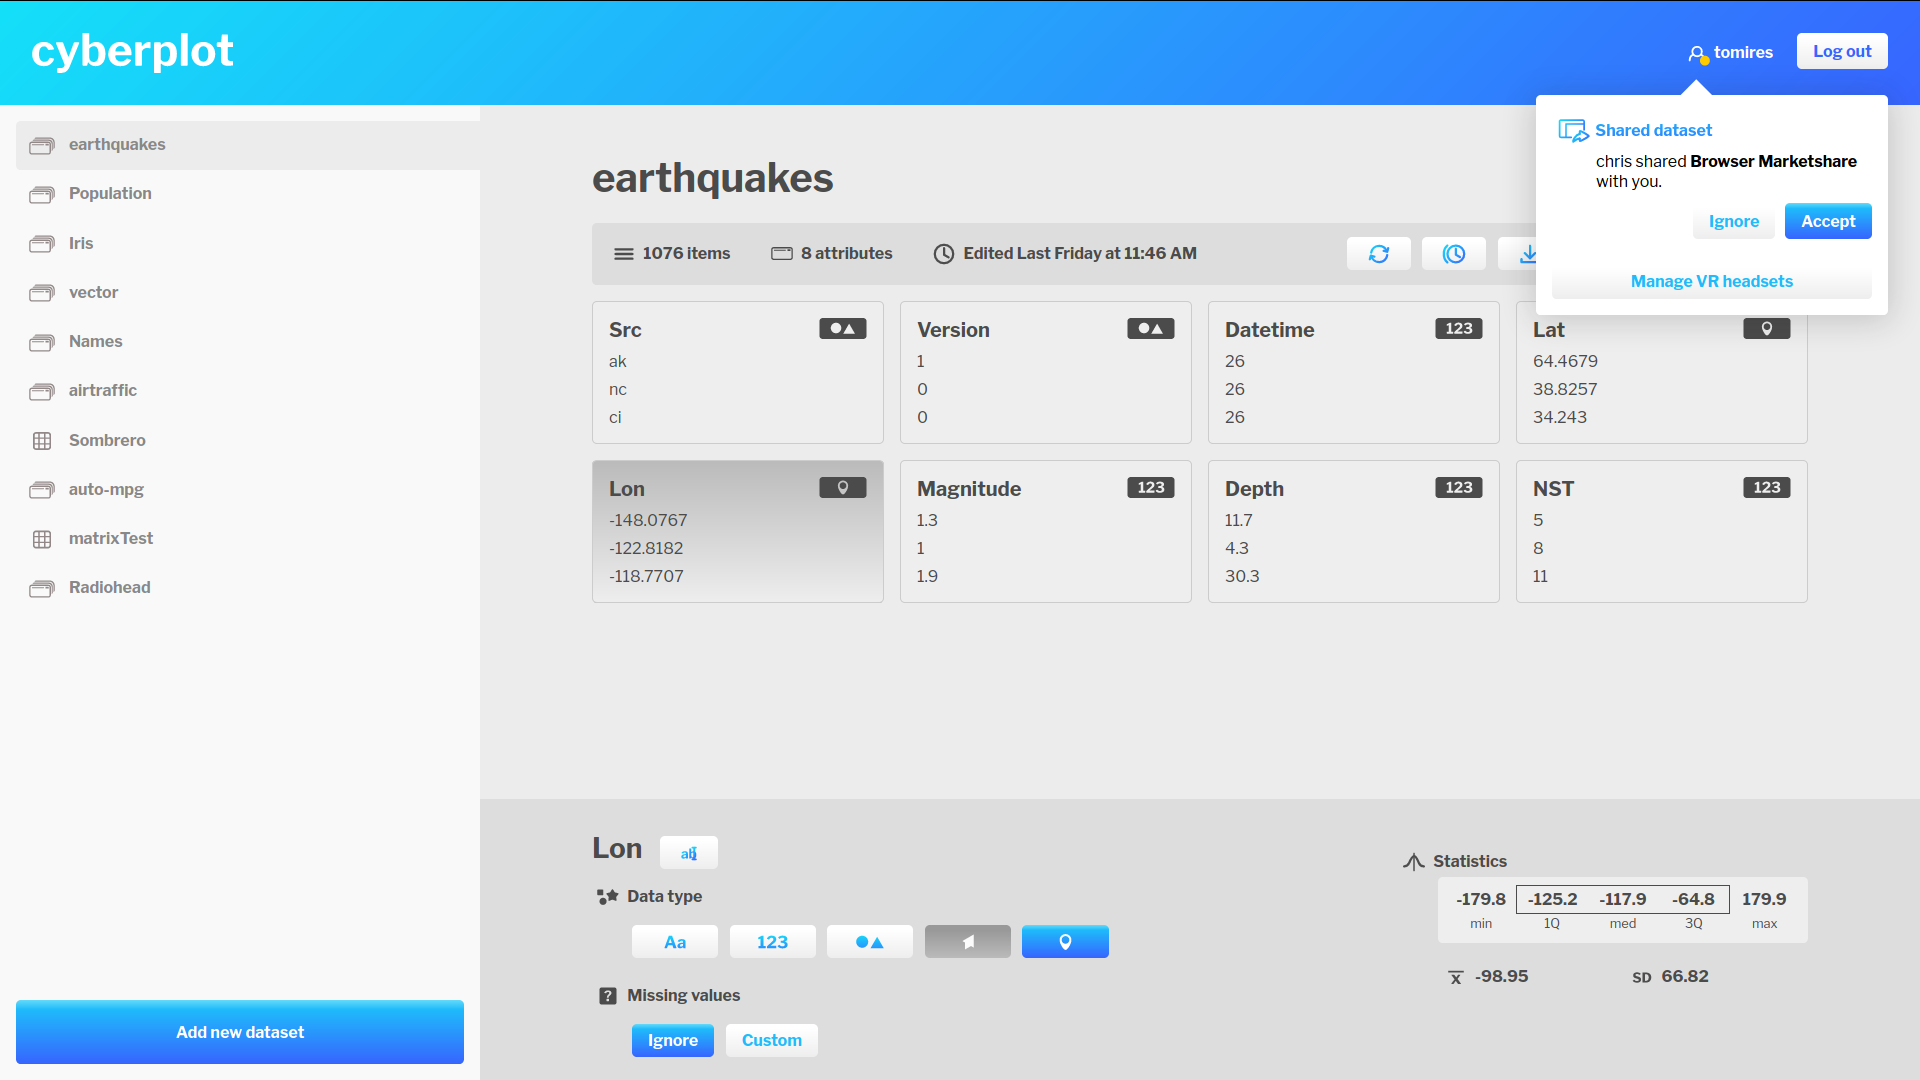
\includegraphics[scale=0.18]{images/manager}
\caption{User interface of Manager.}
\label{fig:manager}
\end{figure}

As it is a multi--user application, the user first has to create an account. After logging in, they are presented with a list of their datasets on a sidebar to the left. In the upper right corner of the screen, they can see their username and access a notification center, which is where they are able to answer share requests and, most importantly, access the VR headset management window. This window gives them information on headsets associated with their account, such as an identifier (name of HMD as well as the computer's domain name if provided by host OS) and time of association.\\

In the lower left corner is a button titled \emph{Add new dataset}. Pressing it opens up a wizard for adding a dataset. The same wizard with slight differences is also used when updating a dataset. In the first step, the user can select their data source. If they choose a programming environment, they receive instructions on how to use the plugin system.\\

\begin{figure}[!h]
\centering
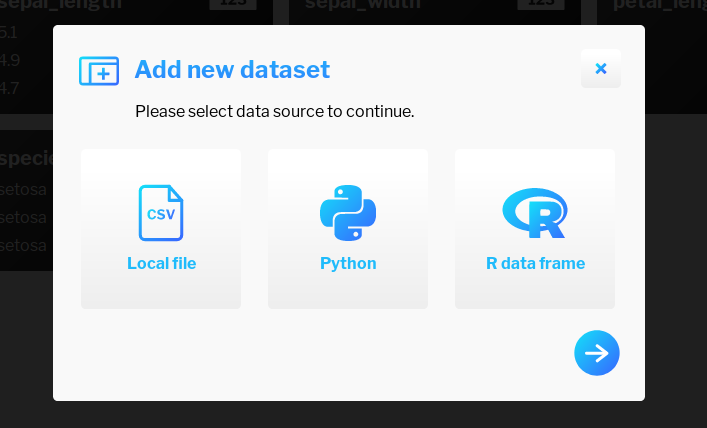
\includegraphics[scale=0.35]{images/manager_add}
\caption{Options for adding a dataset.}
\label{fig:manageradd}
\end{figure}

\newpage

If they choose to create a dataset from local file, they are prompted to select a CSV file by either opening an OS--native file picker dialog or by dragging a file icon into their web browser. In the next step, they have to decide whether the first line of their file includes labels. After selecting an appropriate answer, the dataset is uploaded and appears in the sidebar. Attribute types are assigned automatically.\\

\newpage

\begin{figure}[!h]
\centering
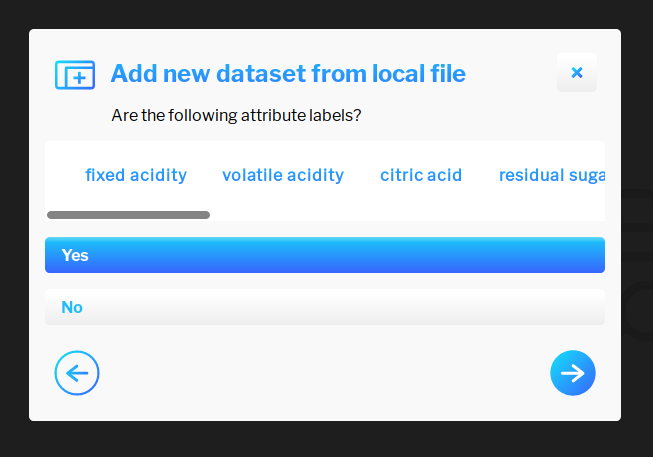
\includegraphics[scale=0.35]{images/manager_labels}
\caption{Dataset addition wizard.}
\label{fig:managerlabels}
\end{figure}

Clicking on a dataset in the sidebar brings up the dataset view, which contains select metadata (number of attributes, row count, timestamp of last edit), buttons for accessing various functions and a listing of all attributes. For each attribute, we can see its label, data type and a preview of its values. Clicking on an attribute brings up the attribute view that contains options to rename an attribute, change its data type (nominal, numerical, categorical, vector) and decide on which action to take in case some values are missing. With numerical attributes, we are able to view select statistical information, such as quartiles, mean and standard deviation.\\

If we return back to dataset--wide actions, we have the following options:

\begin{itemize}
    \item Update dataset
    \item Manage dataset versions
    \item Download dataset file
    \item Share dataset with another user
    \item Rename dataset
    \item Delete dataset
\end{itemize}

\begin{figure}[!h]
\centering
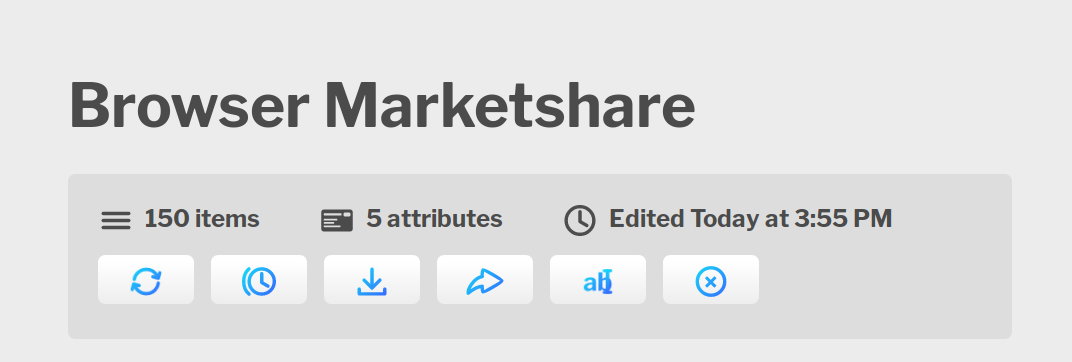
\includegraphics[scale=0.3]{images/manager_actions}
\caption{Dataset actions. From left: Update, manage versions, download, share, rename, delete.}
\label{fig:manageractions}
\end{figure}

Sharing a dataset allows us to select a user with whom to share. The next time they log in, they are presented with a notification that enables them to either accept or decline the share request. Should they accept, the dataset is copied onto their account.\\

\newpage

Datasets can be updated in the same way as they are created, that is using a local file or via the plugin system. The system checks for any type discrepancies and will refuse upload of data incompatible with current attributes. By default, existing data is overwritten on update. However, we can choose to enable versioning in order to keep multiple copies of the same dataset, essentially adding a temporal dimension to our data. Examples of using this feature include a smart device for gathering data, which periodically uploads said data using the plugin system. Versions can be individually downloaded and deleted using the version management interface. Versioning can also be turned on or off on a per dataset basis.\\

\begin{figure}[!h]
\centering
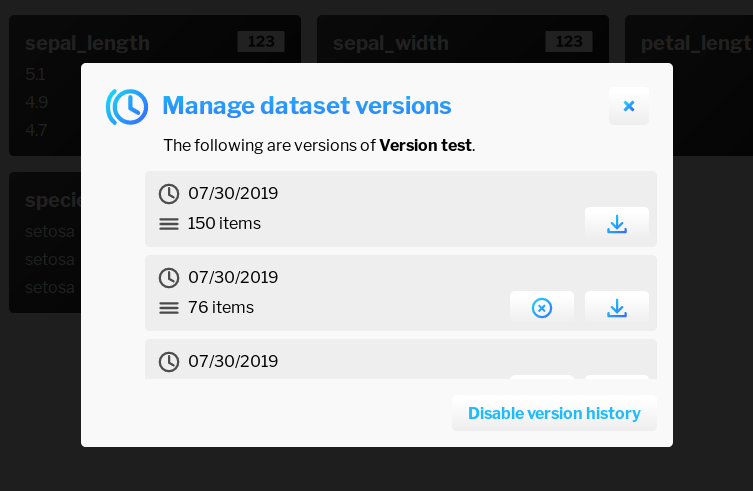
\includegraphics[scale=0.35]{images/manager_versions}
\caption{Version management in Manager.}
\label{fig:managerversions}
\end{figure}

\newpage

\subsubsection{Navigator}

Our VR component is called Navigator. When the user first launches Navigator on their VR headset, they are presented with a 5--digit numeric code, which is used for pairing their account. This system was chosen in order to mitigate poor text input capabilities in virtual reality. Originally, we had planned on using an input solution inspired by a project called Punchkeyboard, however doing so would only work in 6DOF, requiring us to use a traditional keyboard interface in 3DOF.\cite{punchkeyboard} Moreover, we wanted to avoid using text wherever possible as contemporary virtual reality HMDs are still lacking in resolution and text legibility is noticeably impaired on headsets utilizing OLED display technology due to their subpixel arrangement. As such, we try to make maximum use of visual elements.\\

\begin{figure}[!h]
\centering
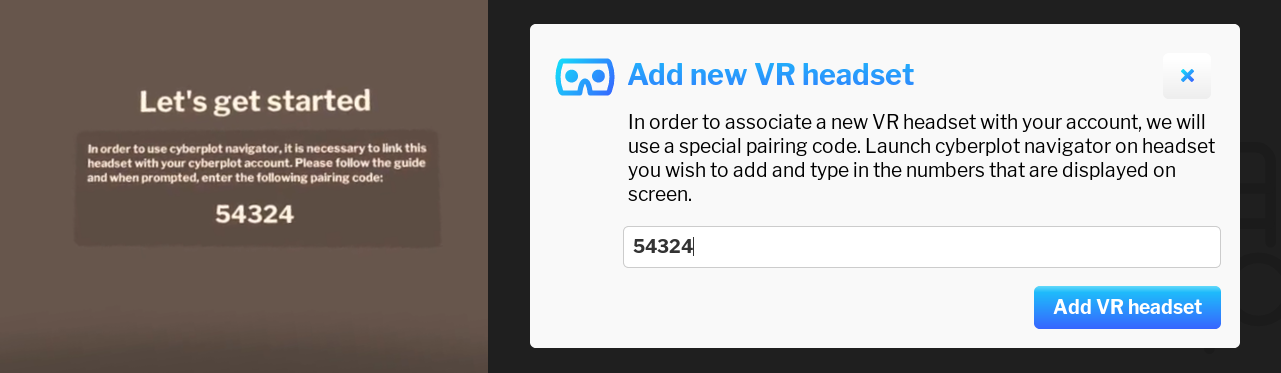
\includegraphics[scale=0.26]{images/pairing}
\caption{Left: Pairing prompt in Navigator. Right: Adding a new headset in Manager.}
\label{fig:pairing}
\end{figure}

After logging in, the user can select one of their datasets, which is then loaded onto what we call a \emph{data brush}, essentially a simplified version of Manager's dataset view. In the 3DOF version, the databrush is present in a fixed position in front of the user's pelvis and while its visibility can be toggled, it is visible for the most part. In the 6DOF version, the user can display the data brush by holding down the grip button. It is then displayed on top of one of their controllers. The data brush displays dataset metadata and attribute listings, which look similar to their Manager counterpart. In order to reduce the amount of text and provide more information, we have opted to display histograms in place of data preview for numerical attributes. The user can move between pages of attributes by utilizing a flick gesture using their controller's analog stick or touchpad. They are also able to switch between versions if versioning is on for selected dataset and load additional datasets. The users are able to have multiple datasets open at the same time.\\

\begin{figure}[!h]
\centering
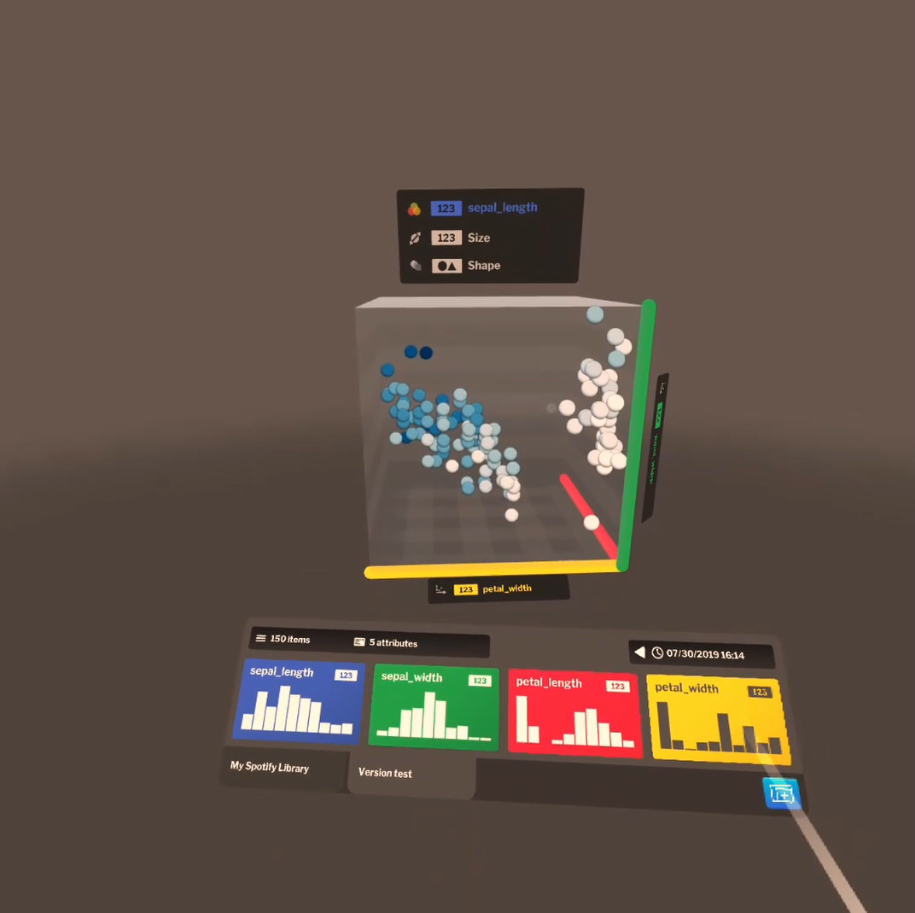
\includegraphics[scale=0.25]{images/cyberplot_3dof.png}
\caption{Navigator's 3DOF interface.}
\label{fig:navigator3dof}
\end{figure}

Plots can be created by pointing at the floor and holding the trigger, which opens up a pie menu with available plot types. Selection can be made by moving the pointer onto an icon and releasing the trigger. This interaction enables the user to quickly create a plot anywhere inside the virtual environment. Plots can be moved around the user's current position by using the trigger and brought closer or further away by using the analog stick or joystick in conjunction with the trigger. If the user drags the plot far away, it turns red and, should the user release the trigger, is deleted from the scene.\\

Plots can also be rotated 90 degrees by pointing at them and using the aforementioned flick gesture. In 3DOF, we try to mitigate the lack of positional movement (which further enhances spatial perception) by offering a free--form rotation mode, which is triggered by pointing at the plot and pressing down on the touchpad. Doing so maps the rotation of a controller onto the rotation of the plot.\\

The plot can also be scaled, although the mechanics differ depending on the VR system used. In 6DOF, one can scale the plot by pointing at it with both controllers, pressing the trigger and dragging inwards or outwards, a fairly standard gesture in VR interface design. In 3DOF we are unable to use this gesture, as most 3DOF systems come with only one controller. We have instead chosen to utilize a twisting motion, where the user twists their wrist in order to control the plot's scale. Such interaction technique had been previously implemented in a VR game \emph{Virtual Virtual Reality}.\cite{vvr}\\

\begin{figure}[!h]
\centering
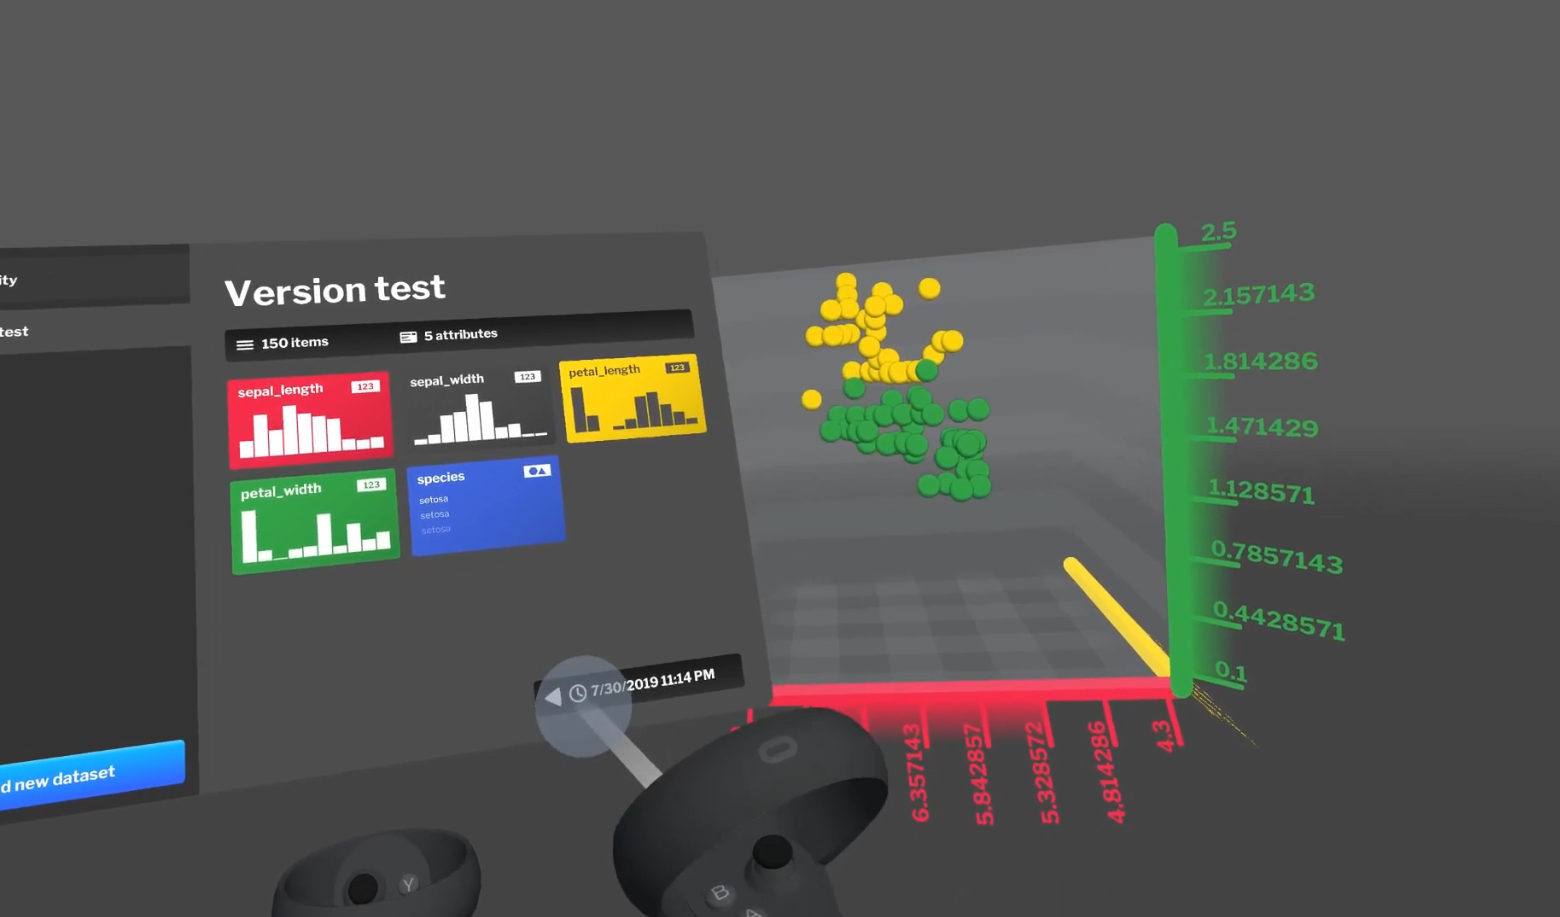
\includegraphics[scale=0.21]{images/cyberplot_6dof.png}
\caption{Navigator's 6DOF interface.}
\label{fig:navigator6dof}
\end{figure}

\newpage

Attributes can be dragged from the data brush onto individual plots by using the trigger button. In the case of scatter plots, they can be assigned to spatial axes and non--spatial features like color and size. When we assign an attribute onto spatial axes, the position of nodes is smoothly interpolated to their new position in order to provide a visual cue to the user. Nodes are depicted as sprites in order to increase performance on mobile hardware. Once an attribute is assigned, it is color--coded on both the plot and the data brush. Color--coding persists until it is removed from all plots. Assignments can be reversed by using the trigger button.\\

Plots also display scales. For numerical attributes we display numerical values for a set number of steps, for categorical attributes, steps are made for each value. The user is able to slice the plot by creating bounds. These are created by pressing on a desired position on a scale.

\section{Used technology}

In this chapter we briefly discuss the technological stack behind our application suite, which consists of a web component called \emph{Manager} and a VR application called \emph{Navigator}. Plugins are omitted, as their implementation varies on the language that they interface with.\\

All user data is stored in Manager and is exposed to Navigator using a set of application programming interfaces (API) adhering to the REST (Representational State Transfer) standard.\cite{fielding}

\subsection{Manager}

Manager consists of a back end written in Flask, a lightweight web application framework for Python.\cite{flask} We make use of a number of Python packages, most notably Numpy\cite{numpy} and Pandas\cite{pandas}, which allow us to extract statistical information from uploaded datasets, and SQLAlchemy, an object--relational mapper (ORM) that enables developers to easily create and manage database schemas directly in Python.\cite{sqlalchemy} In production, we make use of the MySQL database system.\cite{mysql} Front end is written in Vue.js, a JavaScript framework designed for building reactive single--page applications (SPA).\cite{vuejs}

\subsection{Navigator}

Navigator has been written in C\# using Unity game engine.\cite{unity} Unity allows us to deploy on mobile headsets running the Android operating system as well as personal computers running Microsoft Windows, while maintaining a single codebase.\\

In order to support multiple head--mounted units (HMD), we have to target a number of software development kits (SDK), namely Oculus Utilities (Oculus Go, Quest and Rift)\cite{oculusunity}, Microsoft Mixed Reality Toolkit (Windows Mixed Reality headsets)\cite{mrtk} and Valve's OpenVR (HTC Vive, Valve Index).\cite{openvr} While these tools provide some degree of compatibility with headsets from other manufacturers, we have opted to use a wrapper called TButt, which provides abstractions of basic functions for controlling handling and locomotion, greatly reducing complexity of our code.\cite{tbutt}\\

SDK incompatibilities have long been a large issue in VR development, however the release of version 1.0 of Khronos Group's OpenXR at SIGGRAPH 2019 conference held in July 2019 signifies a leap in this area by offering standardized APIs for all HMDs. The specification is supported by all major VR/AR HMD vendors, as well as other stakeholders in the technology space.\cite{openxr}\\

Since we use Unity, we have access to a large number of libraries written for the .NET ecosystem. In our project we utilize a REST client\cite{restclient} that allows us to effortlessly interface with Manager's APIs, as well as an adapted version of SQLite--net called SQLite4Unity3d.\cite{sqliteunity} SQLite, a file--based relational database based on SQL language, is used client--side to store dataset metadata.\cite{sqlite} The aforementioned library was chosen for its support of LINQ, a feature included in modern versions of .NET Framework that allows for easy querying of composite data types.\cite{linq}

\newpage

\section{Testing}

This chapter compares the effeciency of our application against that of its contemporary alternatives introduced in chapter 2. It also outlines the testing methodology.

\subsection{Example task}

The following table lists all KLM operations necessary to complete the task of creating a three--dimensional scatter plot as outlined in the second chapter. It presumes we are logged into Manager and have already associated a VR headset with our account.\\


\begin{table}[!h]
\centering
\caption{Listing of KLM operations for Cyberplot.}
\label{klm-cyberplot}
\scalebox{0.7}{
\begin{tabular}{lll}
Operator & Description & Time (s)\\
M & Initiate opening a file & 1.35\\
M & Find \emph{Add new dataset} button on sidebar & 1.35\\
PB & Point at the button and press it & 1.3\\
PB & Select \emph{Local file} & 1.3\\
PB & Click on \emph{Next} & 1.3\\
PB & Click on \emph{Select file} & 1.3\\
PB & Select file and double click it & 1.3\\
PB & Click on \emph{Next} & 1.3\\
M & Put on the VR headset with Navigator running & 1.35\\
B & Display the data brush by holding the grip button  & 0.2\textsuperscript{6DOF}\\
PB & Point on a dataset and press the trigger & 1.3\\
B & Hide the data brush by releasing the grip button & 0.2\textsuperscript{6DOF}\\
PBPB & Point on the ground, hold trigger, select scatter plot icon, release the trigger & 2.6\\
B & Display the data brush by holding the grip button & 0.2\textsuperscript{6DOF}\\
M & Locate the data brush & 1.35\textsuperscript{3DOF}\\
2*(PBPB) & Drag attributes onto two of the spatial dimensions & 5.2\\
PB & Rotate the plot & 1.3\\
PBPB & Drag an attribute onto the remaining spatial dimension & 2.6\\
PBPB & Drag an attribute onto the color dimension & 2.6\\
B & Hide the data brush by releasing the grip button & 0.2\textsuperscript{6DOF}\\
PB & Point at the scale and press the trigger to slice the plot & 1.3\\
\end{tabular}
}
\end{table}

The total time necessary to complete the tasks is 29.55 seconds for 6DOF and 30.1 seconds for 3DOF versions, considerably faster than with contemporary tools introduced in chapter 2.

\newpage

\subsection{User testing}

We plan to structure our testing sessions in the following order:

\begin{enumerate}
    \item Questionnaire --- section on previous experience.
    \item Introduction to data visualization.
    \item Showcase of ParaView.
    \item Showcase of Tableau.
    \item Questionnaire --- section on traditional tools.
    \item Introduction to Cyberplot.
    \item Demo of Manager and plugins.
    \item Demo of Navigator on Oculus Go (3DOF).
    \item Demo of Navigator on Oculus Rift (6DOF).
    \item Timed tests incorporating all components.
    \item Questionnaire --- Cyberplot--specific section.
\end{enumerate}

Sections 4--5 and 8--9 are going to be conducted in random order in order to mitigate the effects of confounding influences of practice. Participants are to be selected from a diverse range of backgrounds, emphasis is placed on a large variance of experience with virtual reality and the fields of data analysis, statistics and visualization. Timed tests will utilize a modified version of Navigator capable of creating automatic logs and displaying instructions to the user.

\section{Future}

In this chapter we will go over the features that are going to form the focus of future development of our software.

\subsection{Plot types}

So far, we have focused on scatter plots as a means to visualize our data. As part of development, we have also been able to test out bar plots and surface plots, which are going to be released alongside an update to Manager that will add support for data stored in two--dimensional matrices.\\

Additionally, when it comes to multivariate data, we would like to add support for visualizing geospatial data on either a plane or a globe, complete with satellite imagery, as well as support for parallel coordinate plots inspired by the techniques discussed in a related paper.\cite{imaxes}

\begin{figure}[!h]
\centering
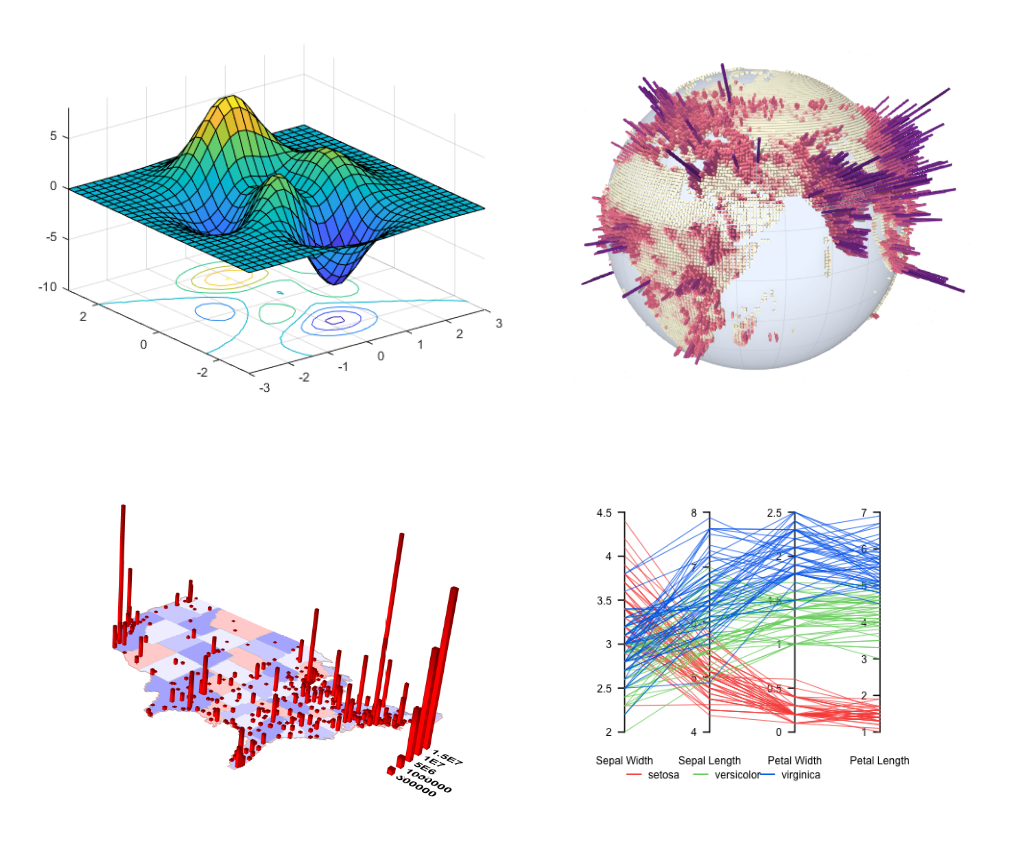
\includegraphics[scale=0.18]{images/plot_types}
\caption{Clockwise from top left: surface plot, bar plot (globe), parallel coordinates plot, bar plot (planar).}
\label{fig:plottypes}
\end{figure}

\subsection{Brushing, linking}

Brushing and linking techniques form an important part of any tool for interactive visualization. Brushing allows the user to select a subset of visualized data items with the goal of either emphasizing or deemphasising it in relation to other data. Linking allows for an extension of this functionality to other plots that are associated with the same dataset.\cite{linking}

\subsection{Sharing system}

As discussed earlier, many similar tools leverage the power of presence in virtual reality to create multi--person sessions, where stakeholders can view and edit data plots and communicate with one another without leaving VR.\\

We plan to utilize an existing solution called Oculus Avatars, which despite its name is available for all major VR platforms.\cite{avatarsdk} We feel that brushing techniques form an integral part of the connected experience and as such, sharing system has a lower priority that the aforementioned features. The feature should allow all stakeholders to interact with visualizations at the same time, unlike ParaView's master--slave approach.

\subsection{Performance optimization}

Due to time constraints, certain dataset--specific analytical functionality had been coded on the Navigator side. These operations are resource--intensive on large datasets and can introduce delays of hundreds of milliseconds on mobile hardware, resulting in somewhat sluggish UI performance. The goal is to move all such functionality to Manager.\\

In addition, it would be advantageous to introduce asynchronicity to the synchronization process that takes place after user opens up Navigator. In its current state, there is a delay of a couple seconds when downloading a large number of datasets.

\subsection{Legend}

It is necessary to implement a plot legend for all non--spatial dimensions. Such UI element needs to be easily accessible, yet unobtrusive. As such we plan to position the element on a user's hand with the capability to show and hide it using a simple wrist twisting gesture akin to looking at a wristwatch.

\begin{figure}[!h]
\centering
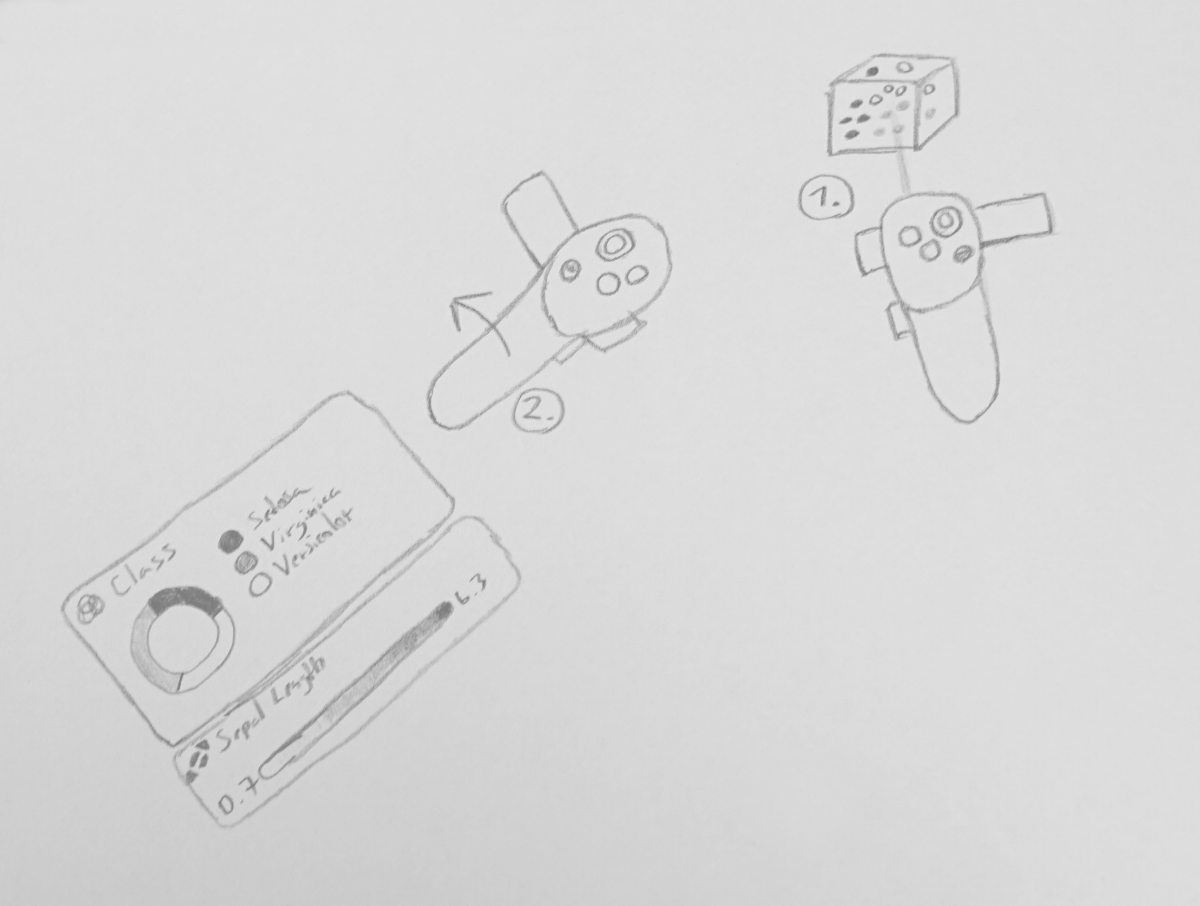
\includegraphics[scale=1.2]{images/legend}
\caption{Sketch of the legend feature. The user points at a plot (1) with one hand and twists the wrist of their other hand (2) to reveal details on all non--spatial features of the plot.}
\label{fig:legend}
\end{figure}

\subsection{Immersion mode}

In order to maximize the benefits of our immersive VR environment, we would like to introduce a so--called \emph{immersion mode}, which would enable users to focus on a single plot while hiding the rest. Immersion mode would come with a brand new control set that would enable users to more effectively view the data. We would also be able to use this mode to render large plots in greater detail (by turning off subsampling) as all other plots would be hidden and thus would not use system resources.

\section{Appendices}

\subsection{Key--stroke level model (KLM)}

\begin{table}[!h]
\centering
\caption{Excerpt of used operators.\cite{klm}}
\label{klm}
\scalebox{0.7}{
\begin{tabular}{lll}
Operator & Description & Time (s)\\
K & Keystroke or button press. & 0.28\footnotemark\\
P & Pointing to a target on a display with a mouse. & 1.1\footnotemark\\
H & Homing the hand(s) on the keyboard or other device. & 0.4\\
M & Mentally preparing for executing physical actions. & 1.35\\
B\footnotemark & Clicking a mouse button. & 0.2
\end{tabular}
}
\end{table}
\footnotetext{Non--secretary typist average (40 words per minute).}
\footnotetext{Average. Varies with distance and target size according to \emph{Fitts's Law}: $t_p = 0.8 + 0.1 * log_2(d / s + 0.5) s$}
\footnotetext{Not present as a separate action in the original paper. Instead it is included as part of the homing motion.}

\subsection{Video transcripts}

The following are transcripts from videos that were created to explain the different parts of our application and also the user interface and controls of our virtual reality component in 3DOF and 6DOF versions.

\subsubsection{Introduction}

Hello, and welcome to Cyberplot, a fresh new way to look at your data. Cyberplot consists of three components --- plugins, Manager and Navigator.\\

You can use plugins to integrate Cyberplot into your programming environment of choice, such as Python or R. Using our API integrations is easy, just follow the instructions.\\

Manager allows you to upload data straight from your computer. This is also where you can edit existing datasets and share them with others.\\

Once you have added some data, it's time to put on your VR headset and launch Cyberplot Navigator. In order to learn more about controls in VR, please watch the next videos in our tutorial series.\\

Ready to get started? Launch Cyberplot Manager by going to the following site and create an account. Next, you will want to associate a headset with your account. When you first launch Navigator, you will be presented with a 5--digit pairing code. Log into Manager and open up the VR headset management window. Enter the pairing code and you're good to go! We'll see you in VR.

\newpage

\subsubsection{6DOF controls}

Hello there. Are you ready to interact with your data in VR? Continue watching to learn the basics of Cyberplot Navigator! In this video, we presume that you are using a headset that includes positional tracking, such as the Oculus Rift, HTC Vive, any of Windows Mixed Reality headsets or the Oculus Quest.\\

After launching into Navigator, hold down the grip button on one of your controllers. Doing so displays what we call a data brush. Start by selecting the dataset that you would like to work with. Your data brush includes basic information about the currently selected dataset as well as listing of all the attributes. Each attribute includes a label, data type and either a histogram or data preview. If there is a larger number of attributes, you can move between pages by moving the analog stick on your controller left or right. Navigator allows you to interact with multiple datasets at the same time. To load a new dataset, click the corresponding button.\\ 

Next, let's learn how to add a plot. Point at the floor and hold the trigger. Move the pointer to a plot type you wish to create and release the trigger. To move the plot around your person, point at it and hold the trigger. You can also move it closer or further away from you by using your controller's analog stick. Make sure you are still holding the trigger while doing so. If you wish to delete the plot, just drag it far away from you and release the trigger. Plots can also be rotated by using the flick gesture we have introduced earlier. In order to resize the plot, select it using both of your controllers and move them apart from one another while holding the trigger buttons.

\subsubsection{3DOF controls}

Hi, and welcome to Cyberplot, a new way to interact with your data in virtual reality. In this video, we will go over controls for headsets that only support rotational tracking like the Oculus Go.\\

After launching into Navigator, you will be presented with a list of all your datasets. Start by selecting the dataset that you would like to work with. You should now be able to see the attributes on what we call a data brush. Your data brush includes basic information about the currently selected dataset as well as listing of all the attributes. Each attribute includes a label, data type and either a histogram or data preview. If there is a larger number of attributes, you can move between pages by swiping the touchpad. Navigator allows you to interact with multiple datasets at the same time. To load a new dataset, click the corresponding button. You can hide your data brush at any time by pressing the back button on your controller. To show the data brush, just press the button again.\\

\newpage

Next, let's learn how to add a plot. Point at the floor and hold the trigger. Move the pointer to a plot type you wish to create and release the trigger. To move the plot around your person, point at it and hold the trigger. You can also move it closer or further away from you by using your controller's touchpad. Make sure you are still holding the trigger while doing so. If you wish to delete the plot, just drag it far away from you and release the trigger. Plots can also be rotated by using the flick gesture we have introduced earlier. You can also enter the freeform rotation mode by pointing on the plot and pressing down on the touchpad. Press the touchpad again, to exit. In order to resize the plot, hold the trigger and twist your wrist like so.

\subsubsection{Shared 3DOF/6DOF}

You now know how to create plots and load datasets. The last thing you need to learn is how to work with attributes. To assign an attribute to a plot, just drag the attribute from the data brush onto one of the axes using the trigger button. You can also map an attribute onto a non--spatial feature of the plot such as color or size. In order to remove an assignment, just click on the attribute's label. You can also change the bounds of selected spatial attributes by clicking on the scales. This is useful for more complex datasets.\\

Lastly, let's learn about versioning. Versioning allows you to keep multiple copies of a single dataset. After enabling versioning inside Cyberplot Manager, you can change between the versions straight from your data brush. And that covers the basics of Cyberplot Navigator. Have fun exploring your data.

\newpage

\section{Used abbreviations}

\begin{table}[!h]
\centering
\caption{Used abbreviations.}
\label{abbreviations}
\scalebox{1}{
\begin{tabular}{ll}
3DOF & 3 degrees of freedom (pitch, yaw, roll)\\
6DOF & 6 degrees of freedom (pitch, yaw, roll, 3D movement)\\
AI & Artificial intelligence\\
API & Application programming interface\\
AR & Augumented reality\\
BI & Business intelligence\\
CSV & Comma--separated values\\
FOSS & Free and open--source software\\
HMD & Head--mounted display\\
IPD & Interpupilary distance\\
KLM & Keystroke--level model\\
LAN & Local area network\\
LINQ & Language Integrated Query\\
OLED & Organic light-emitting diode\\
ORM & Object--relational mapping\\
OS & Operating system\\
PCA & Principal component analysis\\
SDK & Software development kit\\
SPA & Single--page application\\
SQL & Structured Query Language\\
REST & Representational State Transfer\\
UI & User interface\\
VPS & Virtual private server\\
VR & Virtual reality\\
WIMP & Windows--Icons--Menus--Pointing
\end{tabular}
}
\end{table}

\section{Acknowledgements}

I would like to thank all members of the Interactive Content Design Laboratory at Tohoku University for offering a pleasant environment and feedback to my research as well as all past and future volunteers for their patience during testing.

\newpage

\bibliography{bibliography.bib}
\bibliographystyle{IEEEtran}

\end{document}
